\documentclass[12pt,letterpaper]{article}
\usepackage[utf8]{inputenc}
\usepackage[spanish]{babel}
\usepackage[margin=2.5cm]{geometry}
\usepackage{amsmath}
\usepackage{amsfonts}
\usepackage{amssymb}
\usepackage{graphicx} % Paquete necesario para insertar imágenes
\usepackage{comment} % Para poder hacer comentarios

\begin{document}

\begin{center}
    \textbf{\Large Tarea 1: Unidad I}\\
    \vspace{0.2cm}
    \textbf{Física para Ciencias de la Salud (005-1713)}\\
\end{center}

\vspace{0.5cm}
\noindent A continuación se presentan 25 problemas correspondientes a la Unidad I: Relación entre Física y Ciencias de la Salud, distribuidos en ángulos, coordenadas, vectores, potencias de diez y unidades.

\vspace{0.5cm}

\begin{enumerate}

    % === ÁNGULO PLANO ===
    \item \textbf{Ángulo plano (Grados a Radianes):} Un paciente en rehabilitación realiza un movimiento de flexión con su brazo describiendo un ángulo de $60^\circ$. Exprese la medida de este ángulo en radianes.
    \textbf{Solución:} \\
    Para convertir de grados a radianes, multiplicamos por el factor de conversión $\frac{\pi \text{ rad}}{180^\circ}$:
    \[ \theta = 60^\circ \times \left( \frac{\pi}{180^\circ} \right) = \frac{\pi}{3} \text{ rad} \approx 1.047 \text{ rad} \]
    \begin{center}
        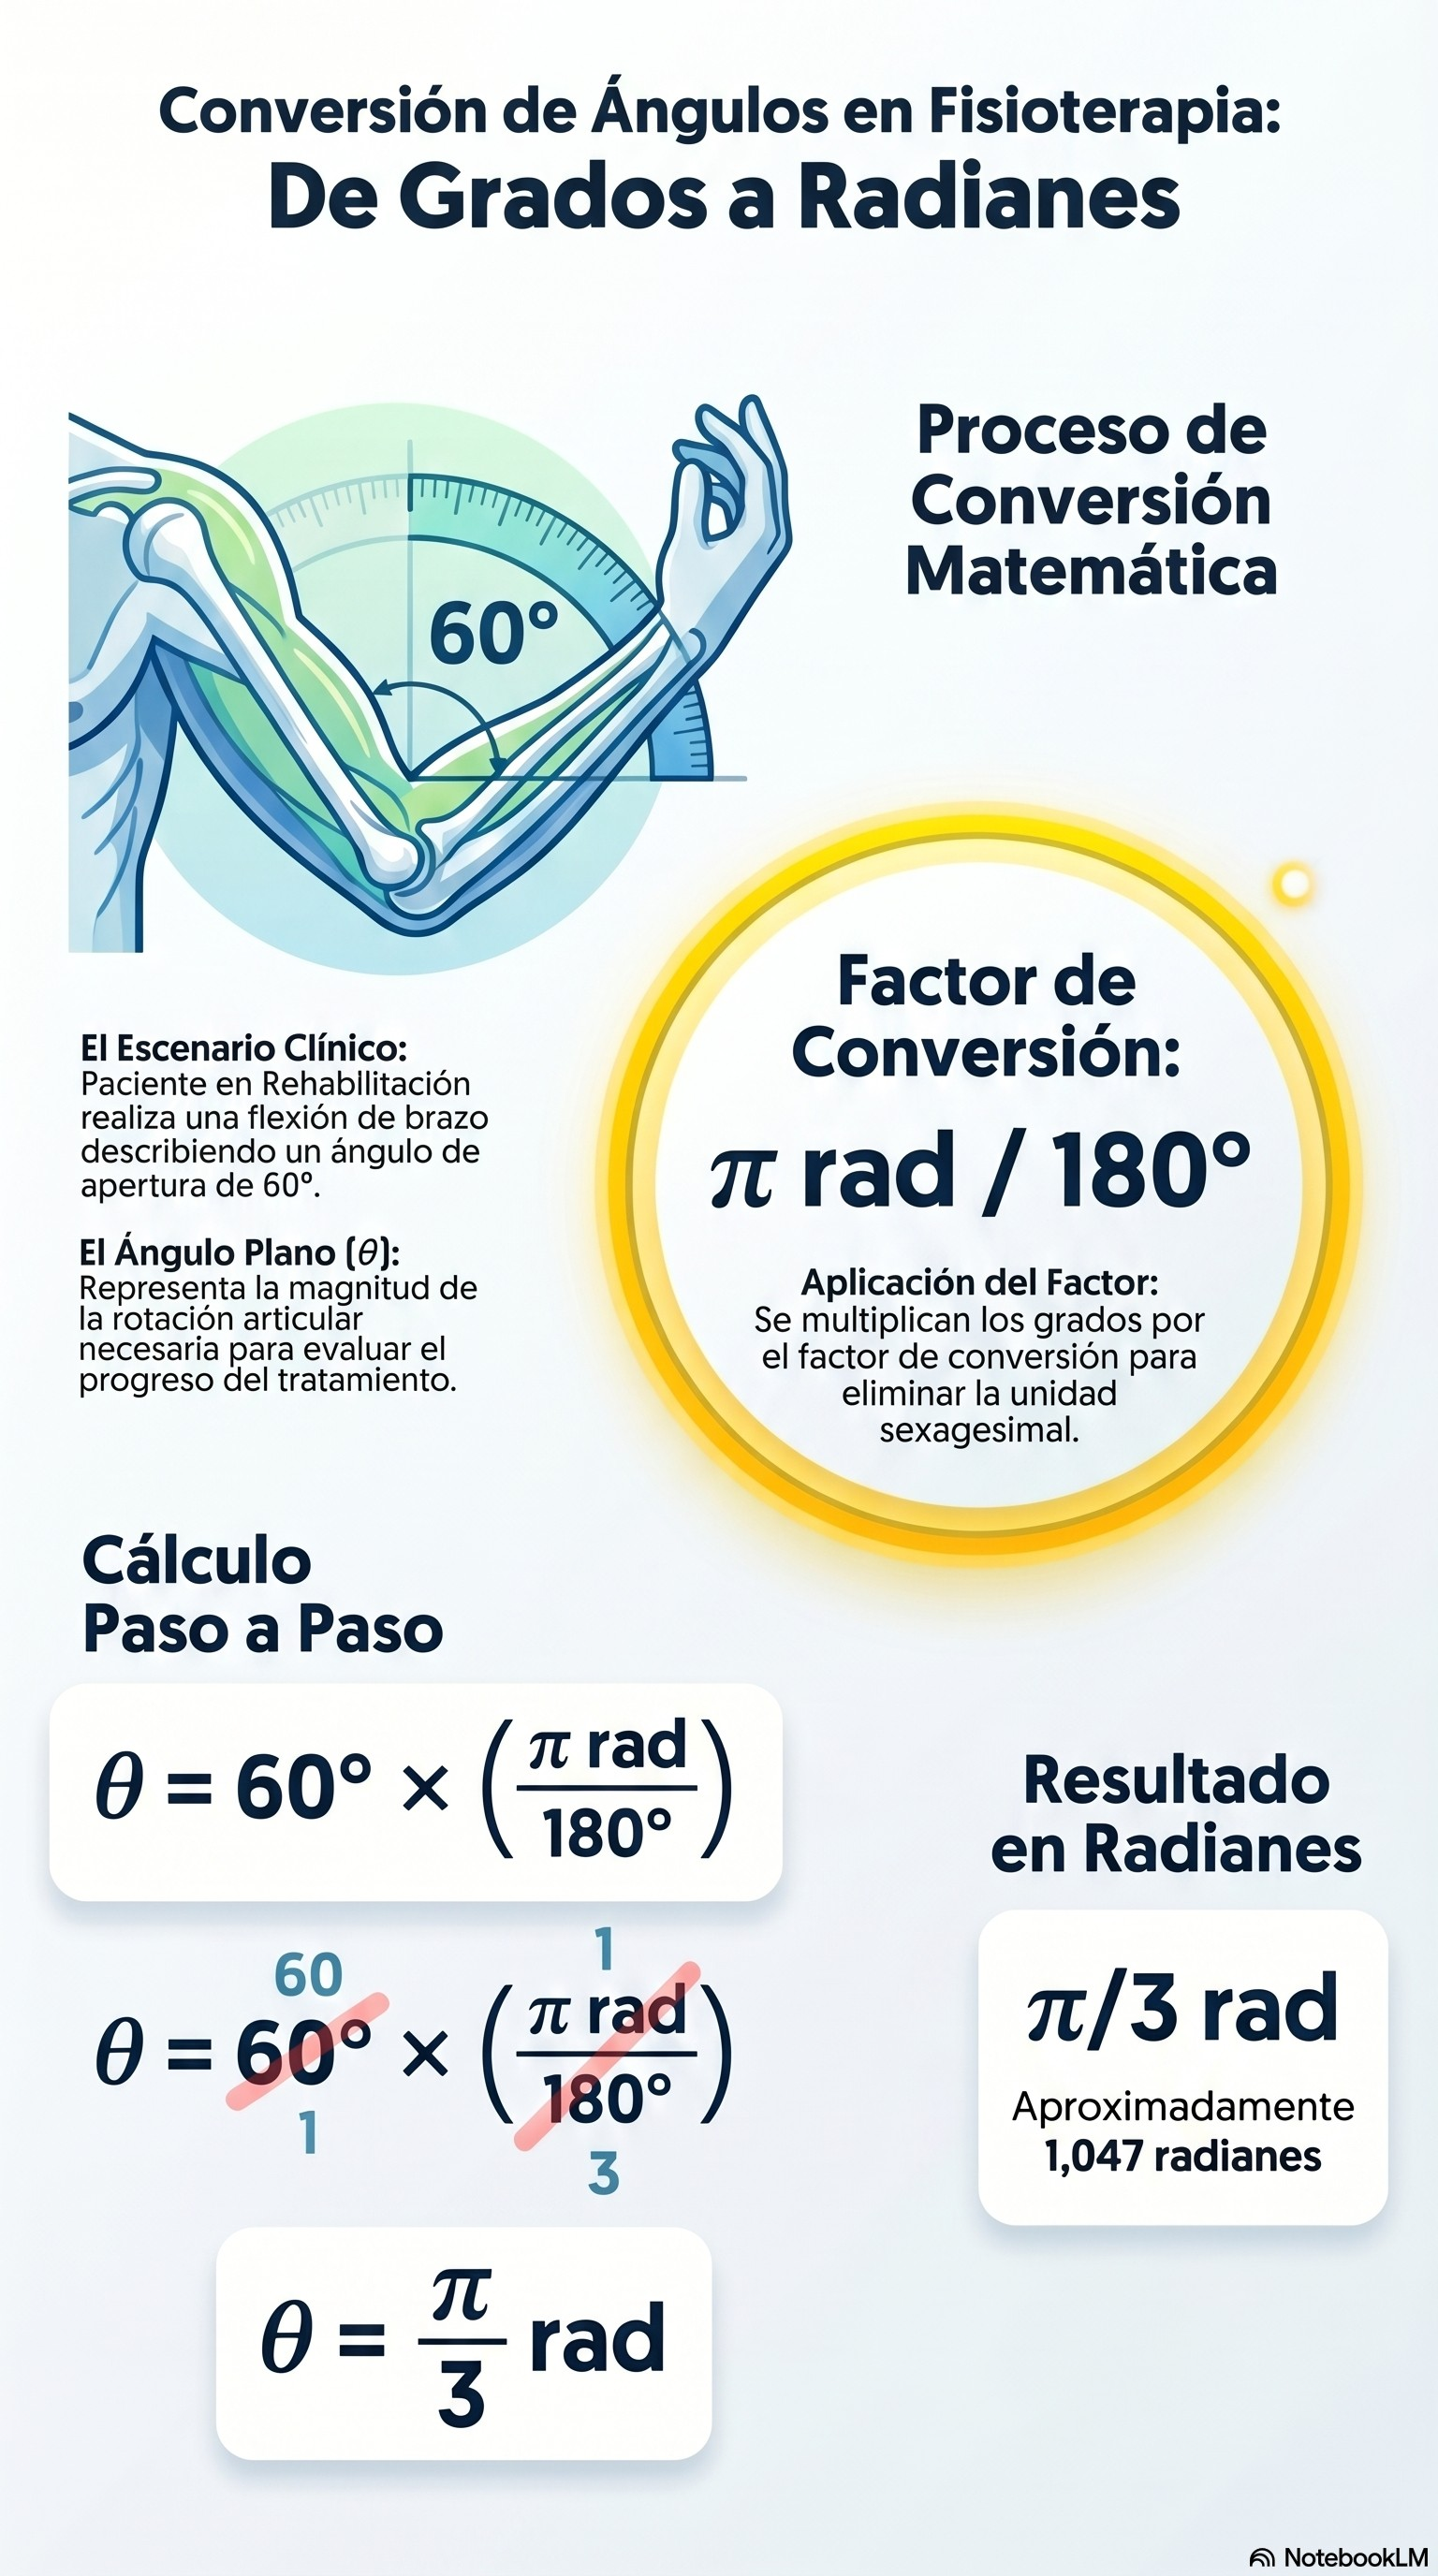
\includegraphics[width=0.6\textwidth]{prob-01.jpg}
    \end{center}
    
    \item \textbf{Ángulo plano (Radianes a Grados):} El campo visual de un microscopio de laboratorio abarca un ángulo de $1.2$ radianes. Convierta este valor a grados sexagesimales.
    \textbf{Solución:} \\
    Se utiliza el factor inverso $\frac{180^\circ}{\pi \text{ rad}}$:
    \[ \theta = 1.2 \text{ rad} \times \left( \frac{180^\circ}{\pi} \right) \approx 68.75^\circ \]
    \begin{center}
        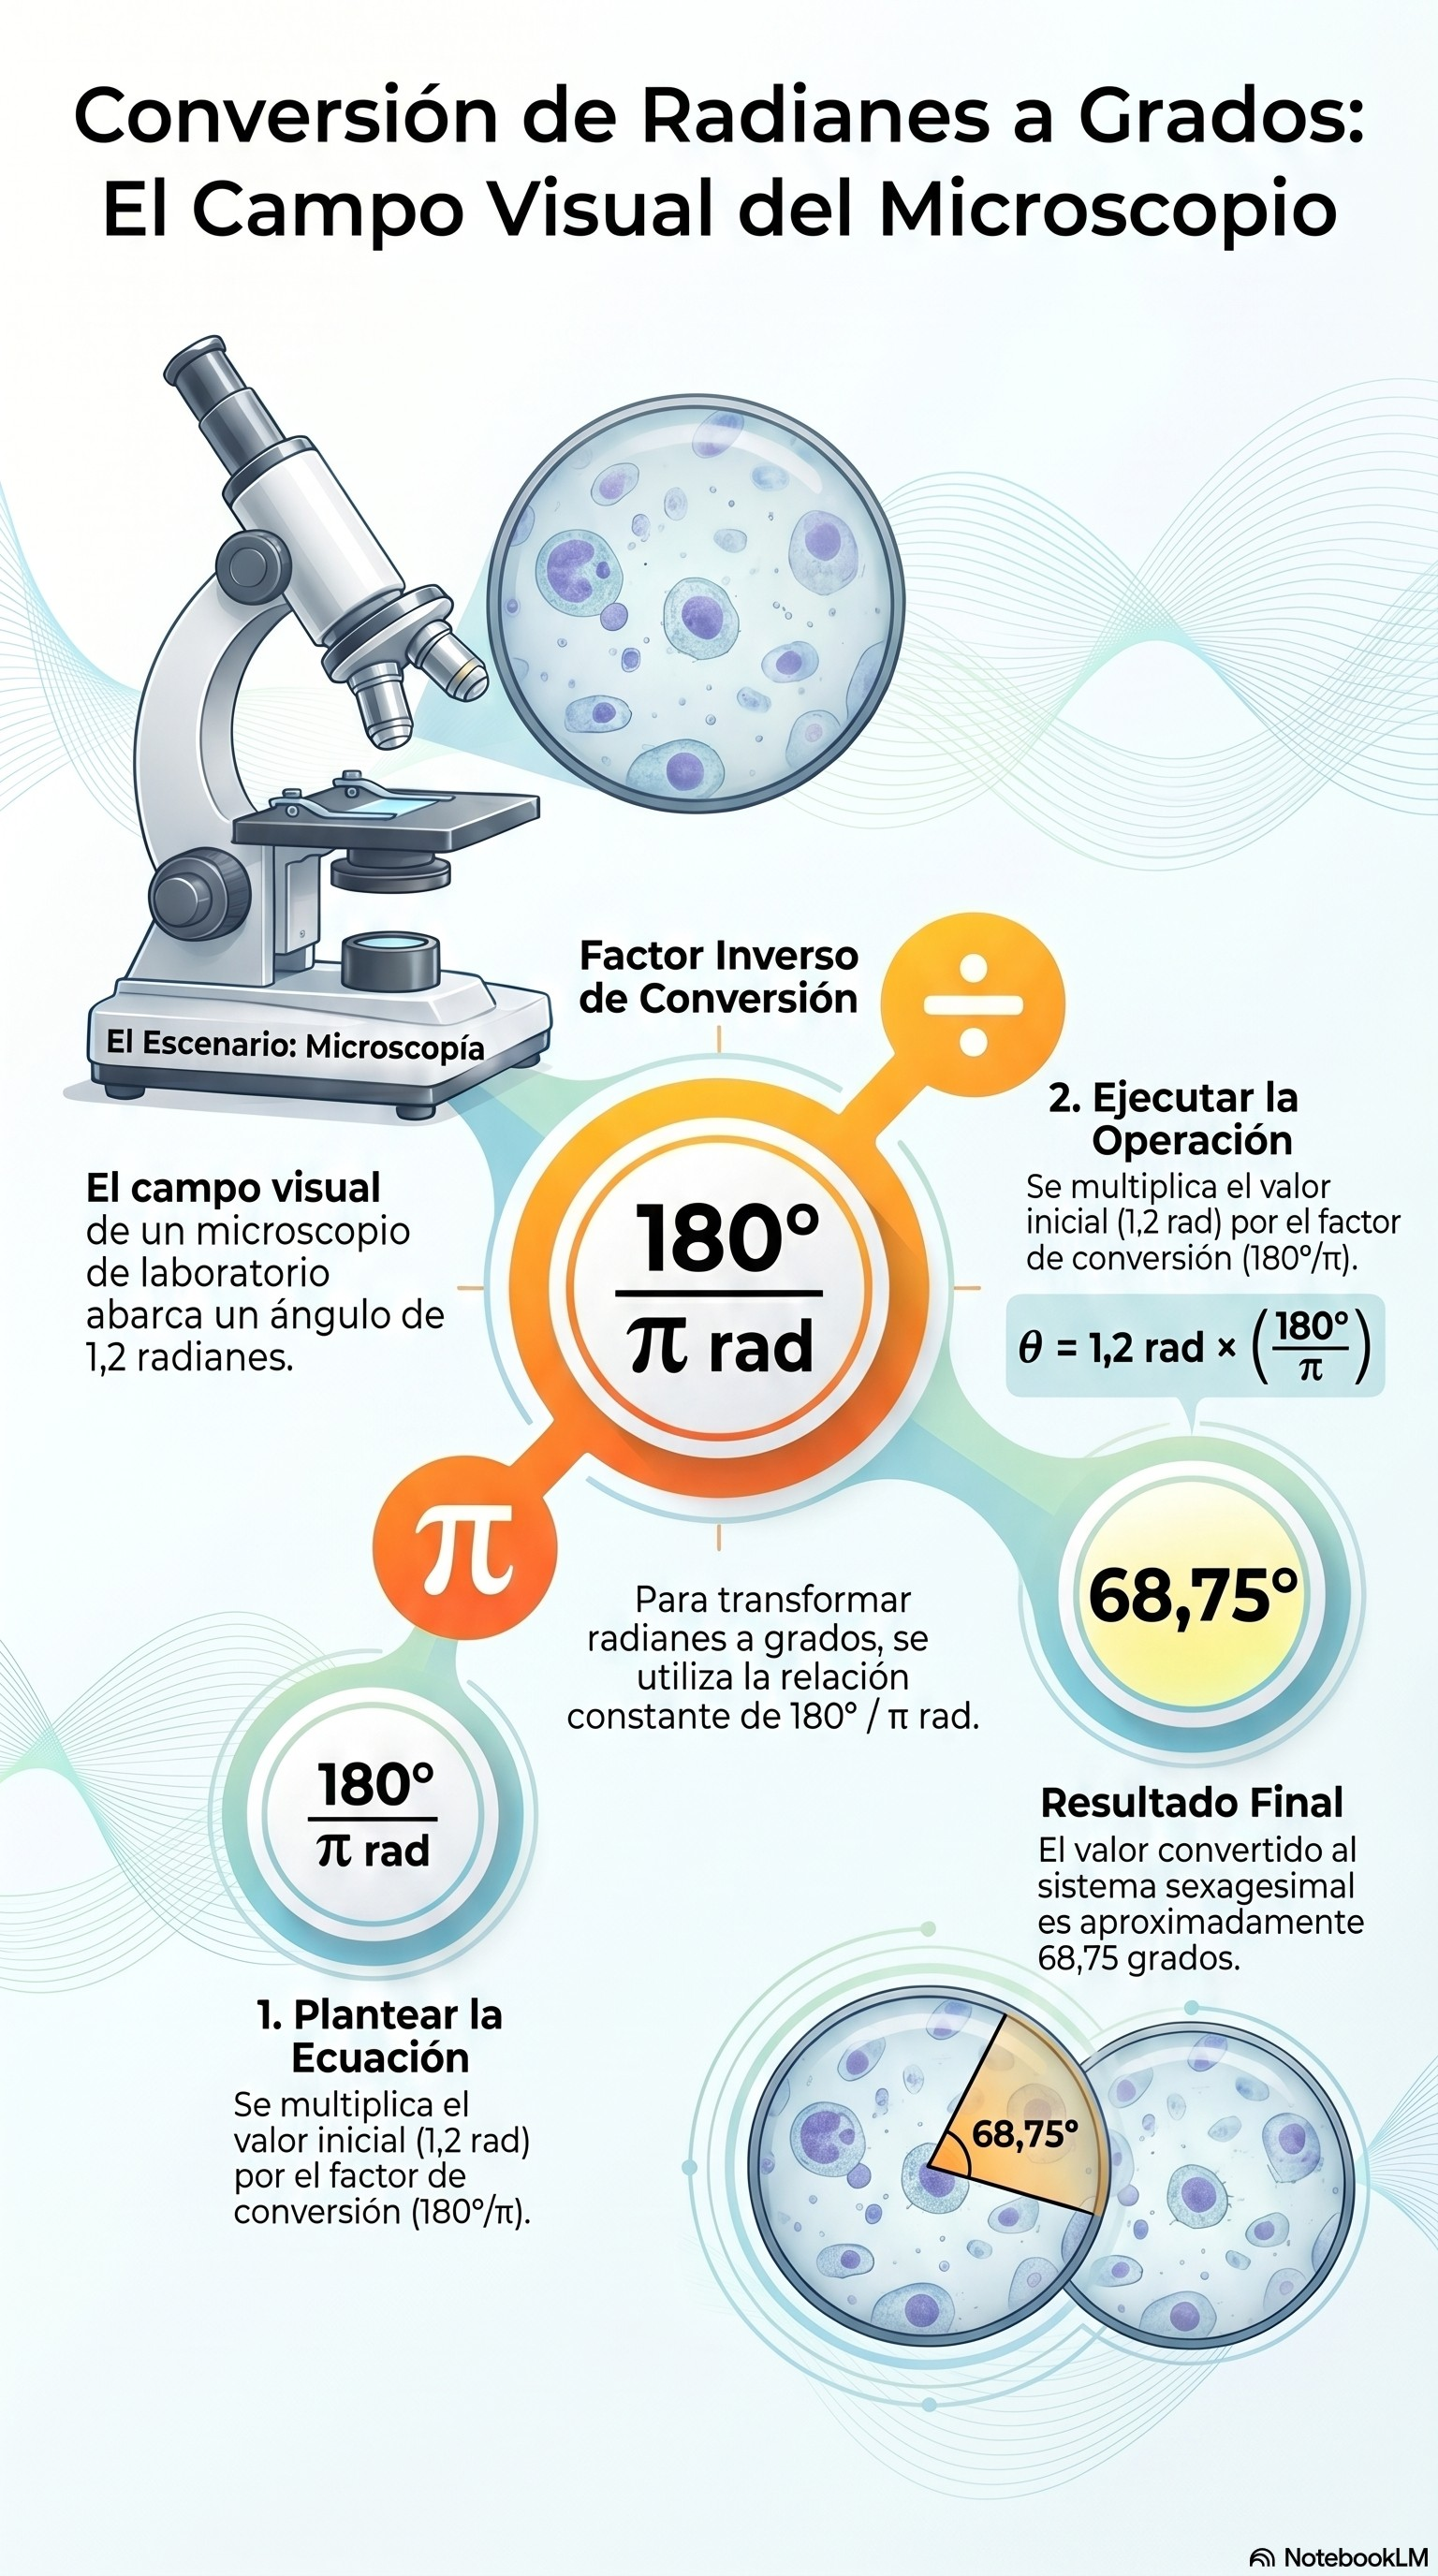
\includegraphics[width=0.6\textwidth]{prob-02.jpg}
    \end{center}
    
    \item \textbf{Ángulo plano (Terapia física):} Durante una terapia de cuello, un paciente logra una rotación lateral equivalente a un ángulo de $\frac{\pi}{4}$ radianes. ¿A cuántos grados corresponde esta rotación?
    \textbf{Solución:} \\
    Multiplicamos por el factor $\frac{180^\circ}{\pi \text{ rad}}$:
    \[ \theta = \frac{\pi}{4} \text{ rad} \times \left( \frac{180^\circ}{\pi} \right) = \frac{180^\circ}{4} = 45^\circ \]
    \begin{center}
        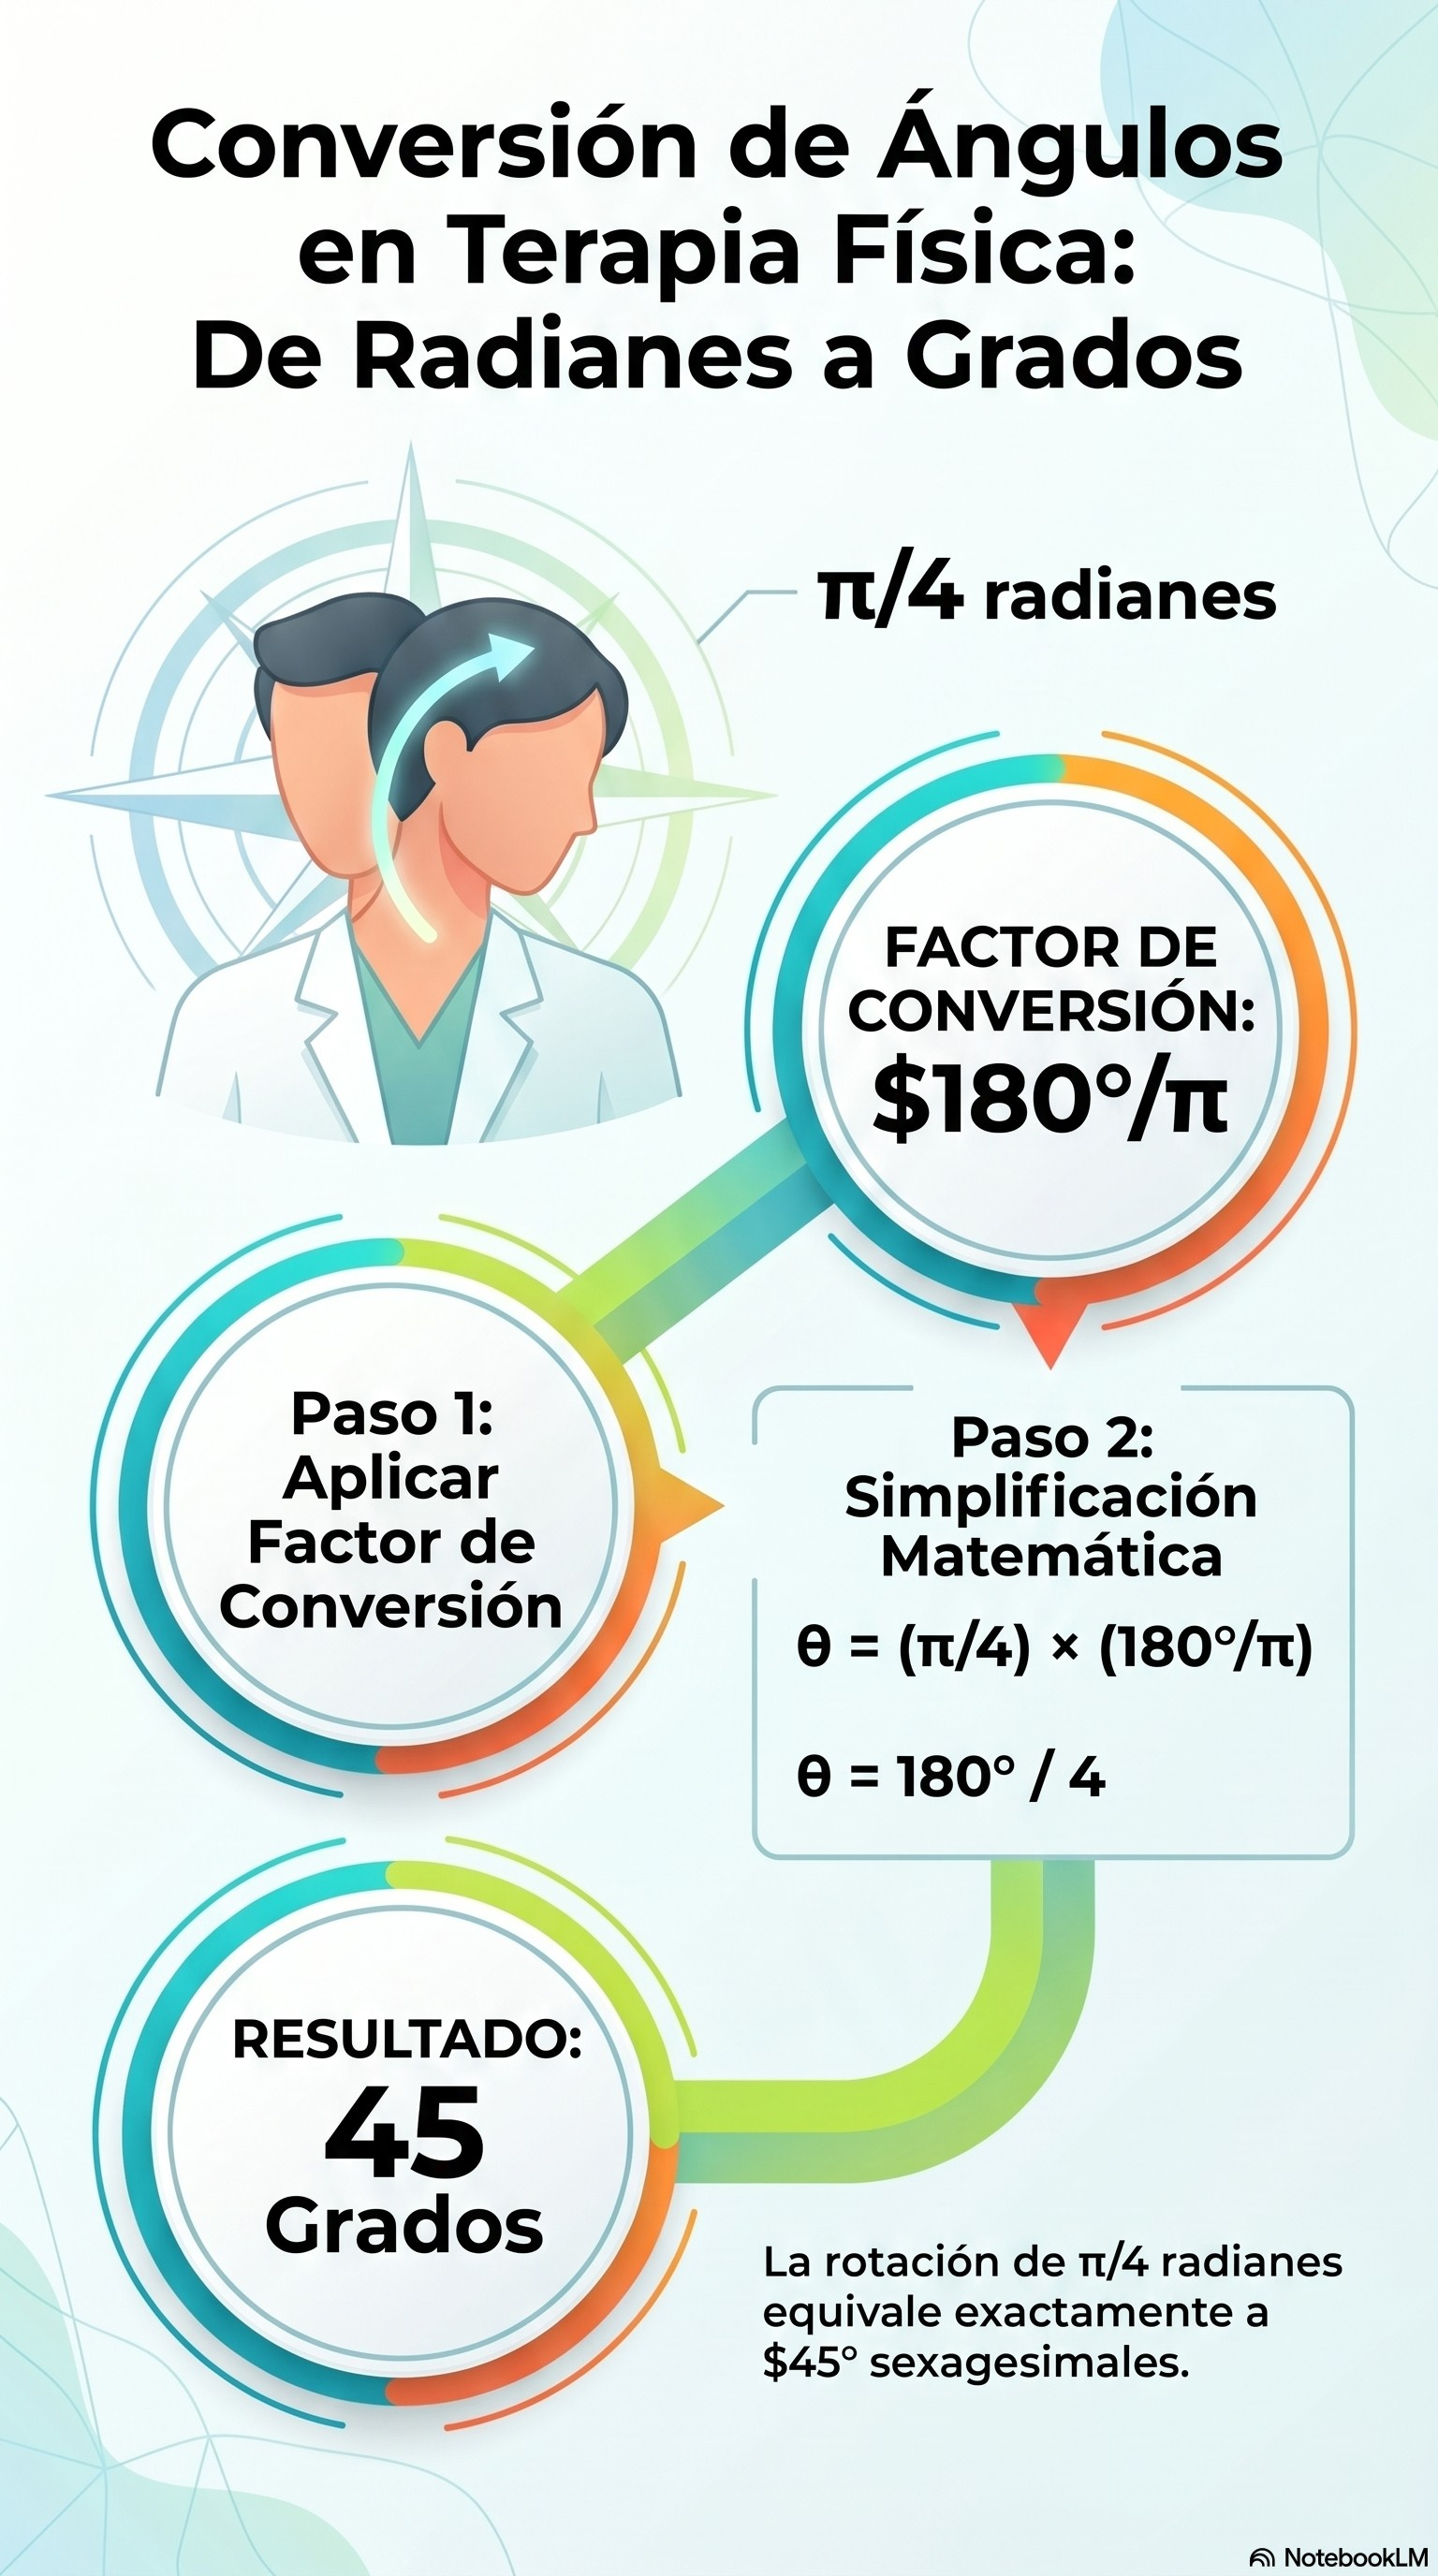
\includegraphics[width=0.6\textwidth]{prob-03.jpg}
    \end{center}
    
    \item \textbf{Ángulo plano (Equipos médicos):} El brazo giratorio de un equipo de tomografía (TAC) escanea a un paciente recorriendo un ángulo de $270^\circ$. Exprese este giro en radianes.
    \textbf{Solución:} \\
    Multiplicamos por el factor de conversión $\frac{\pi \text{ rad}}{180^\circ}$:
    \[ \theta = 270^\circ \times \left( \frac{\pi}{180^\circ} \right) = \frac{3\pi}{2} \text{ rad} = 1.5\pi \text{ rad} \]
    \begin{center}
        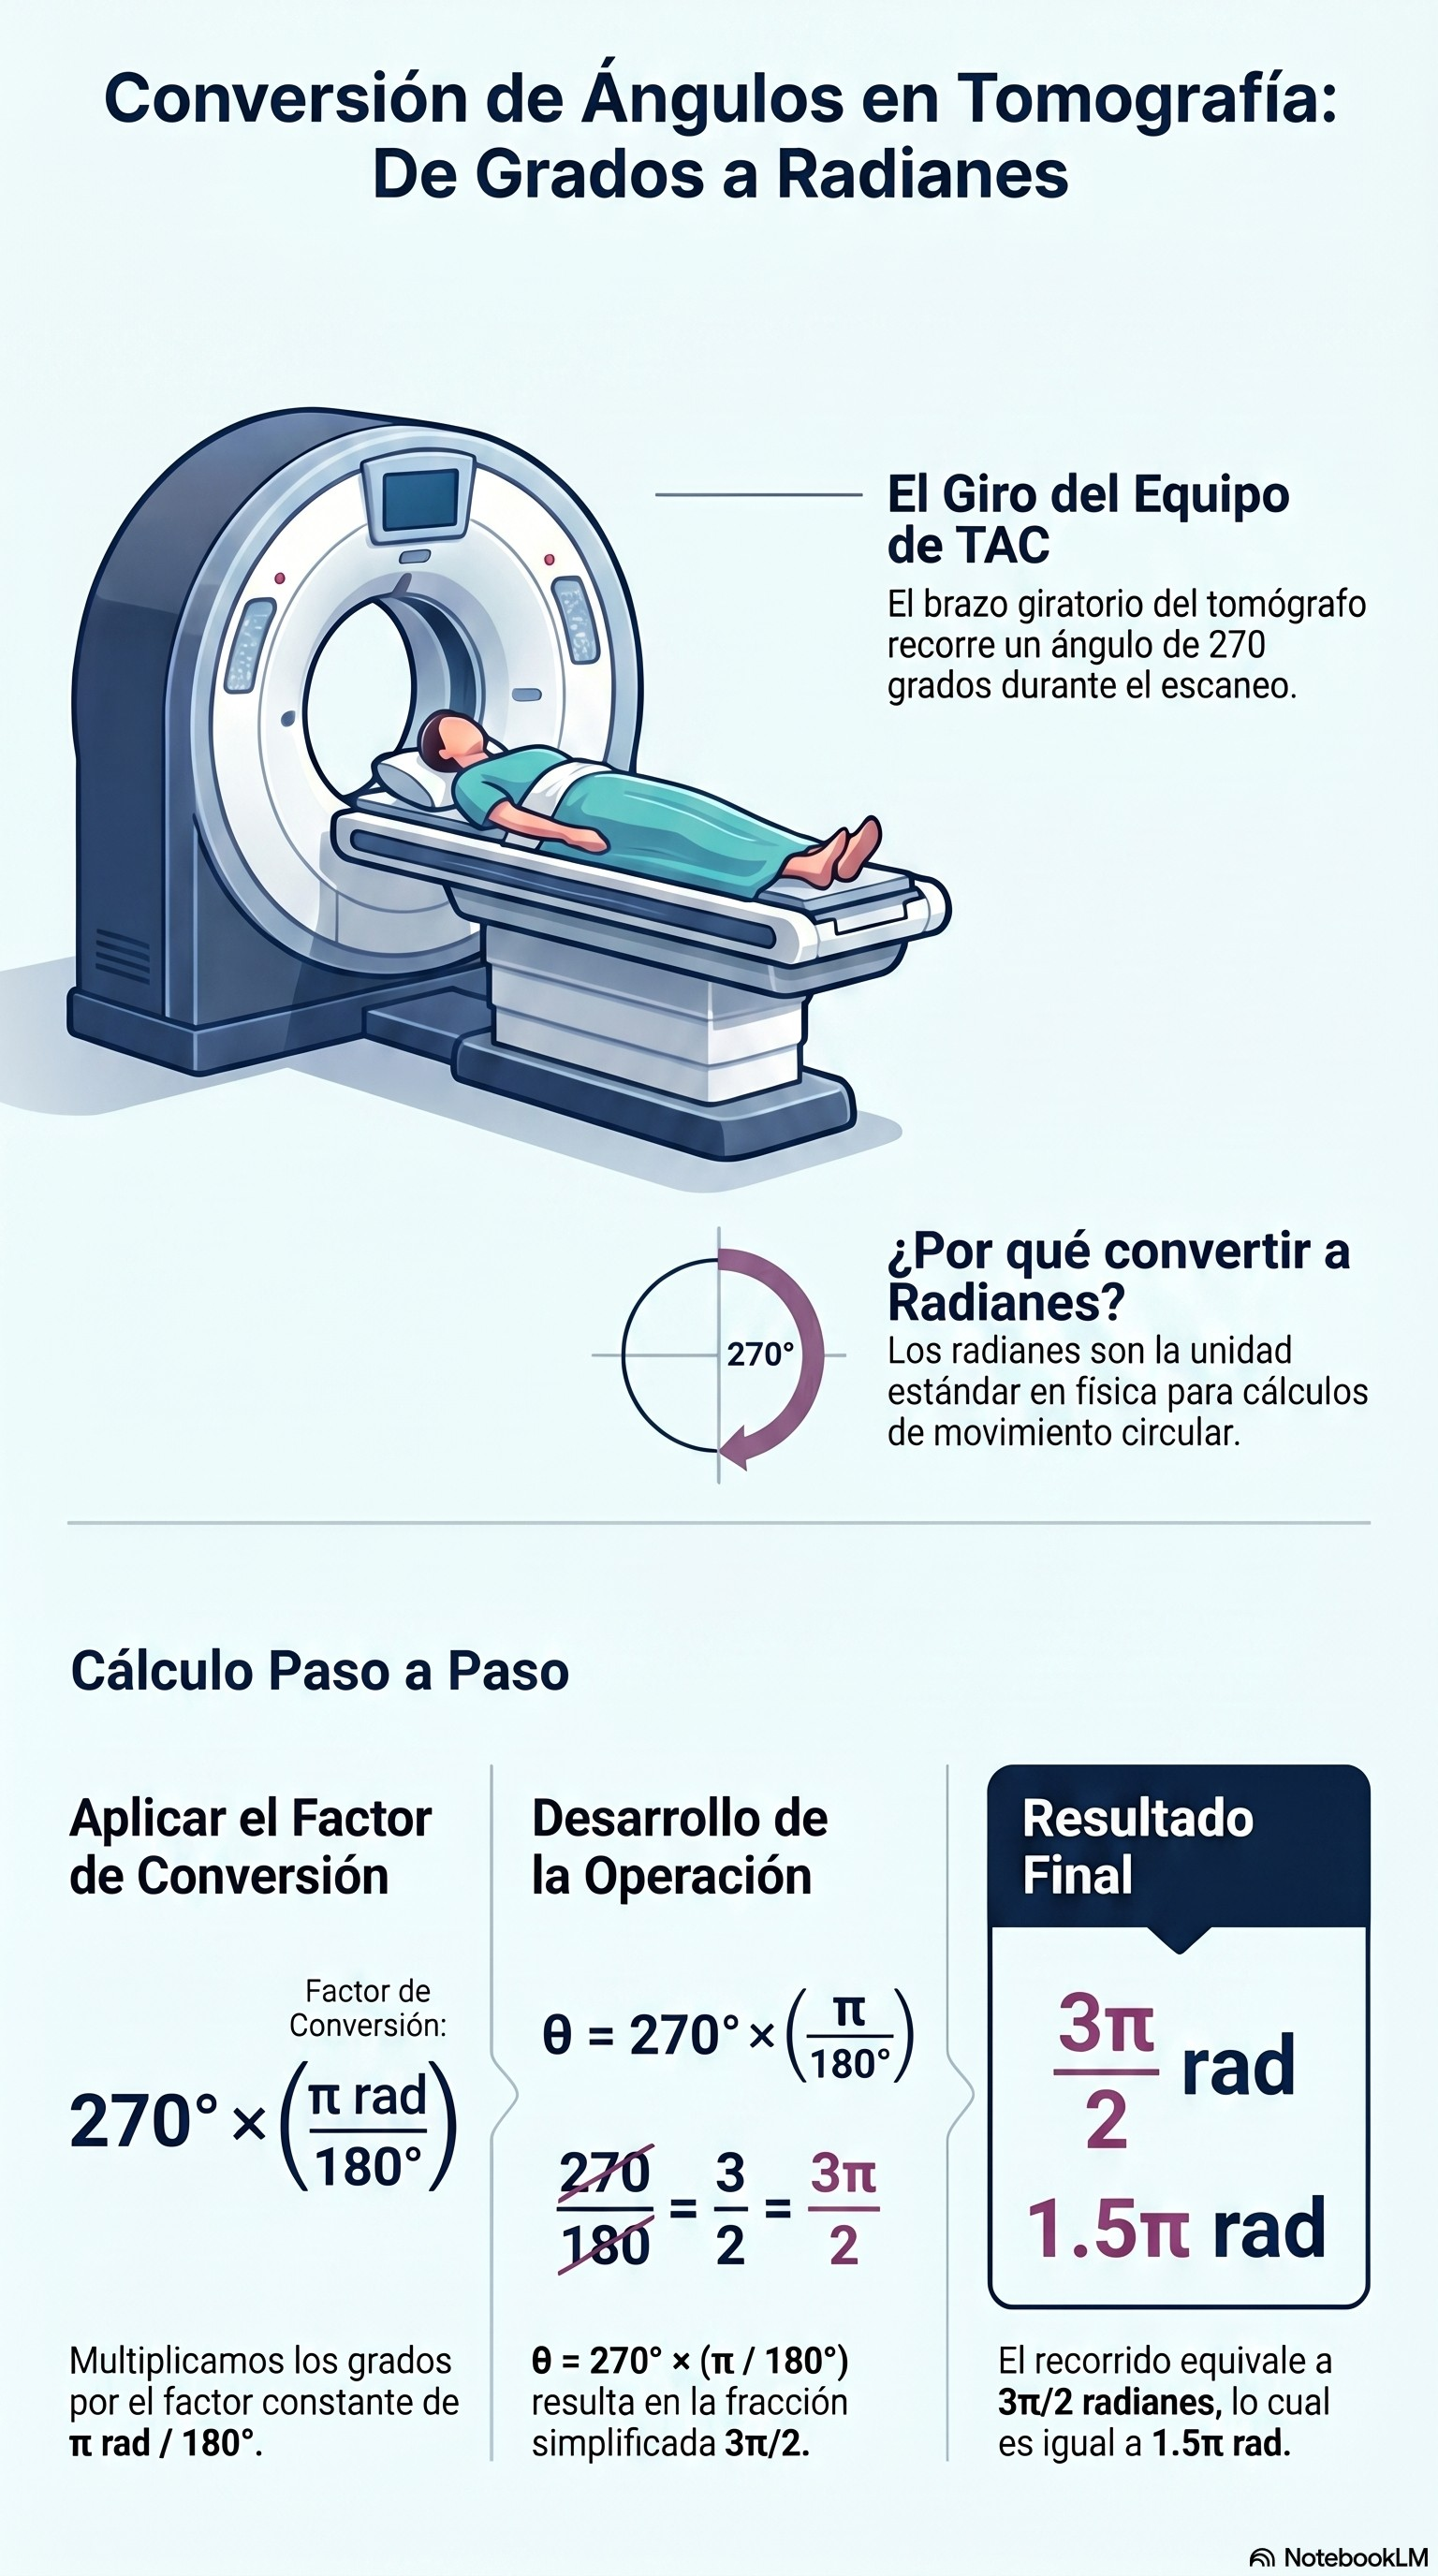
\includegraphics[width=0.6\textwidth]{prob-04.jpg}
    \end{center}
    
    \item \textbf{Ángulo plano (Fisiología articular):} Una extensión de rodilla se mide en $30^\circ$. Determine este ángulo en radianes utilizando factores fraccionarios de $\pi$.
    \textbf{Solución:} \\
    \[ \theta = 30^\circ \times \left( \frac{\pi}{180^\circ} \right) = \frac{30\pi}{180} \text{ rad} = \frac{\pi}{6} \text{ rad} \]
    \begin{center}
        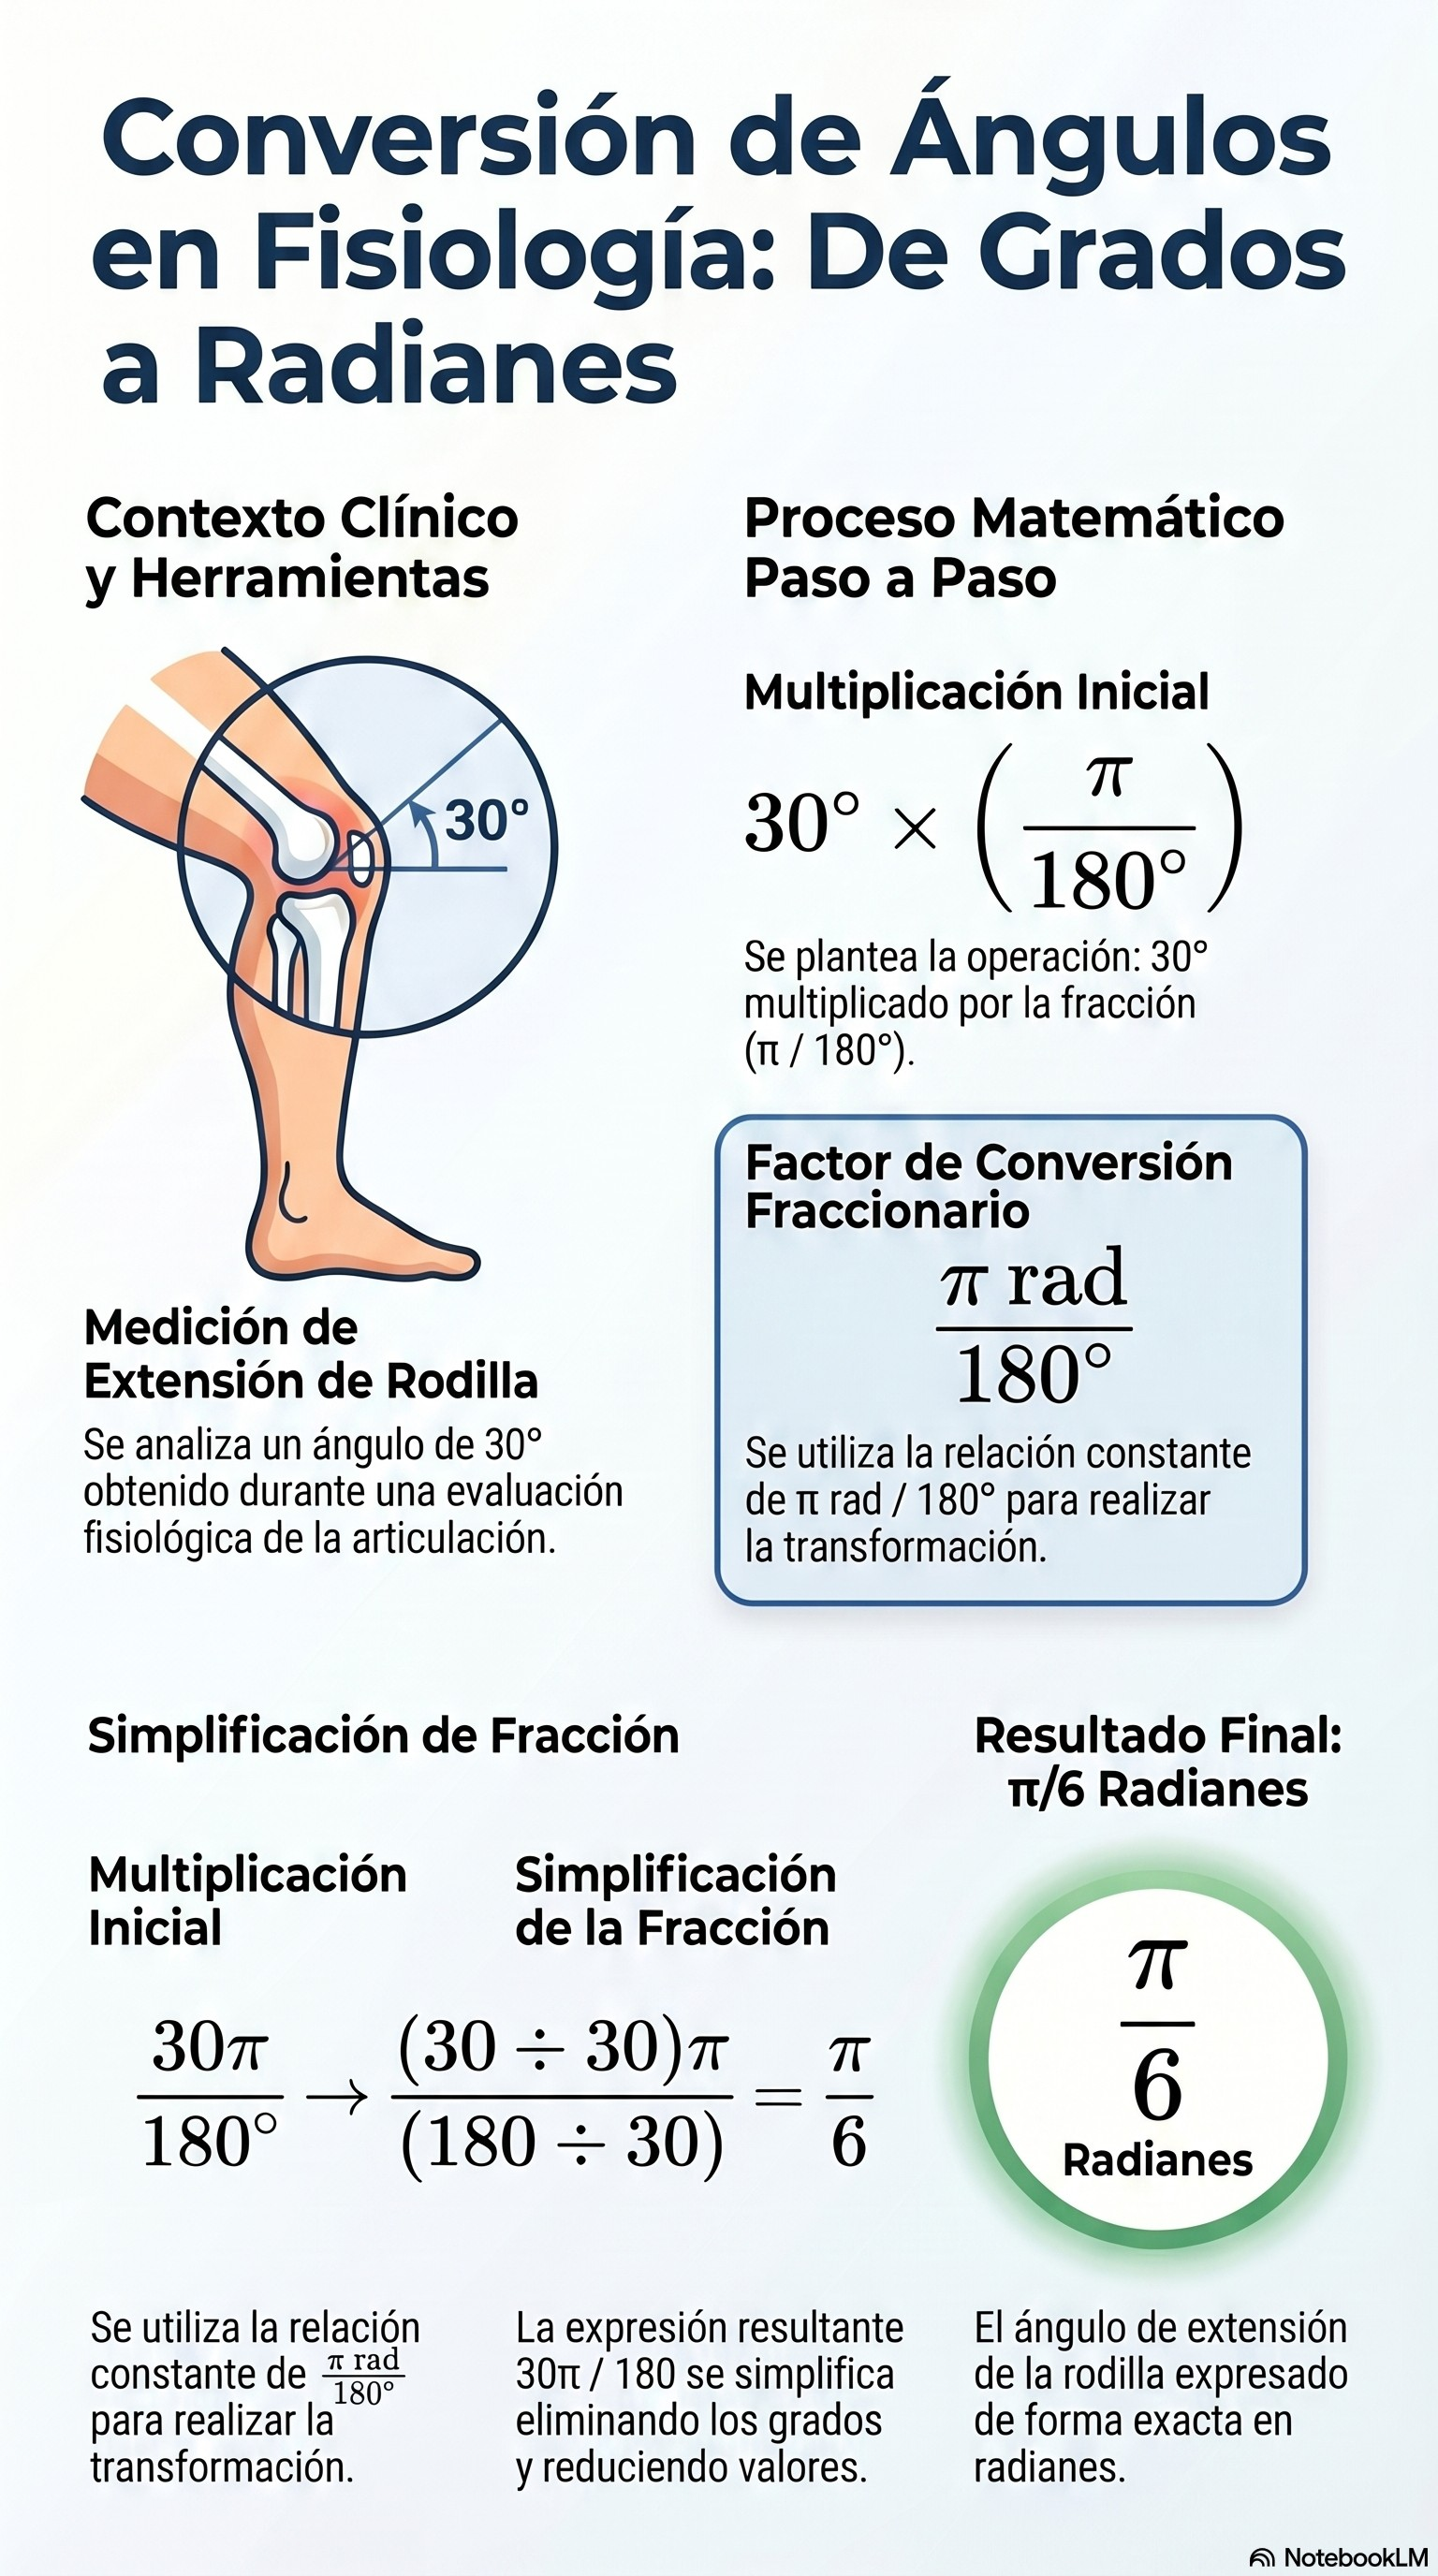
\includegraphics[width=0.6\textwidth]{prob-05.jpg}
    \end{center}

    % === SISTEMAS DE COORDENADAS ===
    \item \textbf{Sistemas de coordenadas (Distancia entre puntos):} En una placa de rayos X digitalizada 2D, el punto de origen de un hueso (articulación A) está en las coordenadas $(2, 3)$ cm y el extremo B en $(5, 7)$ cm. Calcule la longitud real del hueso.
    \textbf{Solución:} \\
    Aplicamos la fórmula de distancia entre dos puntos:
    \[ d = \sqrt{(x_2 - x_1)^2 + (y_2 - y_1)^2} \]
    \[ d = \sqrt{(5 - 2)^2 + (7 - 3)^2} = \sqrt{3^2 + 4^2} = \sqrt{9 + 16} = \sqrt{25} = 5 \text{ cm} \]
    
    \item \textbf{Sistemas de coordenadas (Ubicación de un tumor):} En un mapa cartesiano de un plano sagital de resonancia magnética, el centro de un pequeño tumor benigno se encuentra en $(-2, 4)$ cm y su borde exterior en el punto $(1, 8)$ cm. ¿Cuál es el radio (distancia del centro al borde) del tumor?
    \textbf{Solución:} \\
    Calculamos la distancia entre el centro y el borde:
    \[ r = \sqrt{(1 - (-2))^2 + (8 - 4)^2} = \sqrt{(1 + 2)^2 + (4)^2} = \sqrt{3^2 + 4^2} = \sqrt{9 + 16} = 5 \text{ cm} \]
    
    \item \textbf{Sistemas de coordenadas (Cirugía asistida):} El bisturí de un cirujano robótico se mueve en línea recta desde el punto de origen $(0,0)$ mm hasta las coordenadas $(5, -12)$ mm. Calcule la distancia recorrida en la incisión.
    \textbf{Solución:} \\
    \[ d = \sqrt{(5 - 0)^2 + (-12 - 0)^2} = \sqrt{25 + 144} = \sqrt{169} = 13 \text{ mm} \]
    
    \item \textbf{Sistemas de coordenadas (Electrodos de ECG):} Se colocan dos electrodos en el pecho de un paciente. En un sistema de referencia cartesiano trazado sobre la piel, las posiciones de los electrodos están en $(3, 5)$ cm y $(9, 13)$ cm. Calcule la distancia recta entre ambos.
    \textbf{Solución:} \\
    \[ d = \sqrt{(9 - 3)^2 + (13 - 5)^2} = \sqrt{6^2 + 8^2} = \sqrt{36 + 64} = \sqrt{100} = 10 \text{ cm} \]
    
    \item \textbf{Sistemas de coordenadas (Punto medio):} Durante un análisis forense, se describe una cicatriz que va del punto $A(1, 2)$ cm al punto $B(7, 10)$ cm. Encuentre las coordenadas del punto medio de esta cicatriz.
    \textbf{Solución:} \\
    La fórmula del punto medio es $M = \left(\frac{x_1 + x_2}{2}, \frac{y_1 + y_2}{2}\right)$:
    \[ M = \left(\frac{1 + 7}{2}, \frac{2 + 10}{2}\right) = \left(\frac{8}{2}, \frac{12}{2}\right) = (4, 6) \text{ cm} \]

    % === VECTORES (SUMA Y RESTA) ===
    \item \textbf{Vectores (Suma):} Sobre la vértebra L5 de una persona actúan dos fuerzas debido a la tensión muscular: $\vec{F}_1 = (30\hat{i} + 40\hat{j})$ N y $\vec{F}_2 = (-10\hat{i} + 10\hat{j})$ N. Encuentre el vector de la fuerza resultante que soporta la vértebra.
    \textbf{Solución:} \\
    Sumamos componente a componente:
    \[ \vec{R} = \vec{F}_1 + \vec{F}_2 = (30 - 10)\hat{i} + (40 + 10)\hat{j} = 20\hat{i} + 50\hat{j} \text{ N} \]
    \begin{center}
        \includegraphics[width=0.6\textwidth]{prob-11.png}
    \end{center}
    
    \item \textbf{Vectores (Resta):} Un sistema ortopédico ejercía una tracción inicial $\vec{T}_1 = (50\hat{i} + 20\hat{j})$ N. Después de reajustar los pesos, la tracción es $\vec{T}_2 = (30\hat{i} + 40\hat{j})$ N. Calcule el vector de cambio de fuerza $\Delta\vec{T} = \vec{T}_2 - \vec{T}_1$.
    \textbf{Solución:} \\
    Restamos los vectores componente por componente:
    \[ \Delta\vec{T} = (30 - 50)\hat{i} + (40 - 20)\hat{j} = -20\hat{i} + 20\hat{j} \text{ N} \]
    \begin{center}
        \includegraphics[width=0.6\textwidth]{prob-12.png}
    \end{center}
    
    \item \textbf{Vectores (Desplazamiento por resta):} En una placa de Petri, un leucocito se mueve desde una posición inicial $\vec{r}_1 = (2\hat{i} + 3\hat{j}) \, \mu\text{m}$ hacia una bacteria ubicada en $\vec{r}_2 = (7\hat{i} + 15\hat{j}) \, \mu\text{m}$. Encuentre el vector desplazamiento $\vec{d} = \vec{r}_2 - \vec{r}_1$ y su magnitud.
    \textbf{Solución:} \\
    \[ \vec{d} = (7 - 2)\hat{i} + (15 - 3)\hat{j} = 5\hat{i} + 12\hat{j} \, \mu\text{m} \]
    Su magnitud es $|\vec{d}| = \sqrt{5^2 + 12^2} = \sqrt{25 + 144} = \sqrt{169} = 13 \, \mu\text{m}$.
    \begin{center}
        \includegraphics[width=0.6\textwidth]{prob-13.png}
    \end{center}
    
    \item \textbf{Vectores (Suma de múltiples fuerzas):} Tres pequeñas bandas elásticas ejercen fuerza en una articulación de los dedos durante terapia ocupacional: $\vec{F}_1 = 10\hat{i}$ N, $\vec{F}_2 = 5\hat{j}$ N, y $\vec{F}_3 = (-2\hat{i} + 3\hat{j})$ N. Calcule la fuerza total resultante.
    \textbf{Solución:} \\
    Agrupamos todas las componentes en $x$ e $y$:
    \[ \vec{R} = (10 + 0 - 2)\hat{i} + (0 + 5 + 3)\hat{j} = 8\hat{i} + 8\hat{j} \text{ N} \]
    
    \item \textbf{Vectores (Suma y ajuste):} Para neutralizar un desgarro muscular que tira con una fuerza de $\vec{F}_m = (25\hat{i} - 15\hat{j})$ N, un fisioterapeuta aplica una fuerza restauradora $\vec{F}_r = (-25\hat{i} + 15\hat{j})$ N. Demuestre matemáticamente el estado de equilibrio (Suma de fuerzas = 0).
    \textbf{Solución:} \\
    \[ \vec{F}_{\text{total}} = \vec{F}_m + \vec{F}_r = (25 - 25)\hat{i} + (-15 + 15)\hat{j} = 0\hat{i} + 0\hat{j} = 0 \text{ N} \]

    % === POTENCIAS DE DIEZ ===
    \item \textbf{Potencias de diez (Notación Científica):} Un glóbulo rojo (eritrocito) humano tiene un diámetro aproximado de $0.0000075$ metros. Exprese esta medida utilizando notación científica (potencias de diez) y el prefijo adecuado del Sistema Internacional.
    \textbf{Solución:} \\
    Movemos la coma decimal 6 lugares a la derecha:
    \[ d = 7.5 \times 10^{-6} \text{ m} \]
    Sabiendo que el prefijo para $10^{-6}$ es micro ($\mu$), la medida es $7.5 \, \mu\text{m}$ (micrómetros).
    
    \item \textbf{Potencias de diez (Multiplicación):} La concentración de un determinado fármaco en la sangre es de $3 \times 10^{-4}$ moles por litro. Si el volumen total de sangre de un paciente contiene este fármaco disperso en $5 \times 10^0$ litros, ¿cuántos moles del fármaco hay en total en el torrente sanguíneo?
    \textbf{Solución:} \\
    Multiplicamos la concentración por el volumen:
    \[ \text{Total de moles} = (3 \times 10^{-4} \text{ moles/L}) \times (5 \times 10^0 \text{ L}) \]
    Agrupando los coeficientes y las potencias de base 10:
    \[ (3 \times 5) \times (10^{-4} \times 10^0) = 15 \times 10^{-4} = 1.5 \times 10^{-3} \text{ moles} \]
    
    \item \textbf{Potencias de diez (Masas pequeñas):} La masa de un virus común se estima en $0.00000000000000001$ kg. Exprese esta medida en notación científica.
    \textbf{Solución:} \\
    Movemos el punto decimal 17 lugares a la derecha hasta ubicarlo tras el 1:
    \[ m = 1 \times 10^{-17} \text{ kg} \]
    
    \item \textbf{Potencias de diez (Cantidades grandes):} Los pulmones humanos contienen un promedio de 480,000,000 de alvéolos para el intercambio gaseoso. Escriba esta cifra empleando potencias de diez.
    \textbf{Solución:} \\
    Movemos el punto decimal 8 lugares hacia la izquierda:
    \[ \text{N}^{\circ} \text{ Alvéolos} = 4.8 \times 10^8 \]
    
    \item \textbf{Potencias de diez (Biomasa celular):} En un cultivo de laboratorio, se cuenta una colonia de bacterias con $2 \times 10^6$ individuos. Si se asume que cada bacteria tiene una masa de $1 \times 10^{-12}$ gramos, ¿cuál es la masa total de la colonia?
    \textbf{Solución:} \\
    Multiplicamos cantidad por masa individual:
    \[ M = (2 \times 10^6) \times (1 \times 10^{-12} \text{ g}) = (2 \times 1) \times 10^{6 + (-12)} = 2 \times 10^{-6} \text{ g} = 2 \, \mu\text{g} \]

    % === SISTEMAS DE UNIDADES ===
    \item \textbf{Sistemas de unidades (Densidad):} En un análisis de laboratorio, se determina que la densidad de una muestra de sangre es de $1.06 \, \text{g/cm}^3$. Convierta este valor a las unidades estándar del Sistema Internacional ($\text{kg/m}^3$).
    \textbf{Solución:} \\
    \[ \rho = 1.06 \, \frac{\text{g}}{\text{cm}^3} \times \left( \frac{1 \text{ kg}}{1000 \text{ g}} \right) \times \left( \frac{10^6 \text{ cm}^3}{1 \text{ m}^3} \right) = 1060 \, \frac{\text{kg}}{\text{m}^3} \]
    \begin{center}
        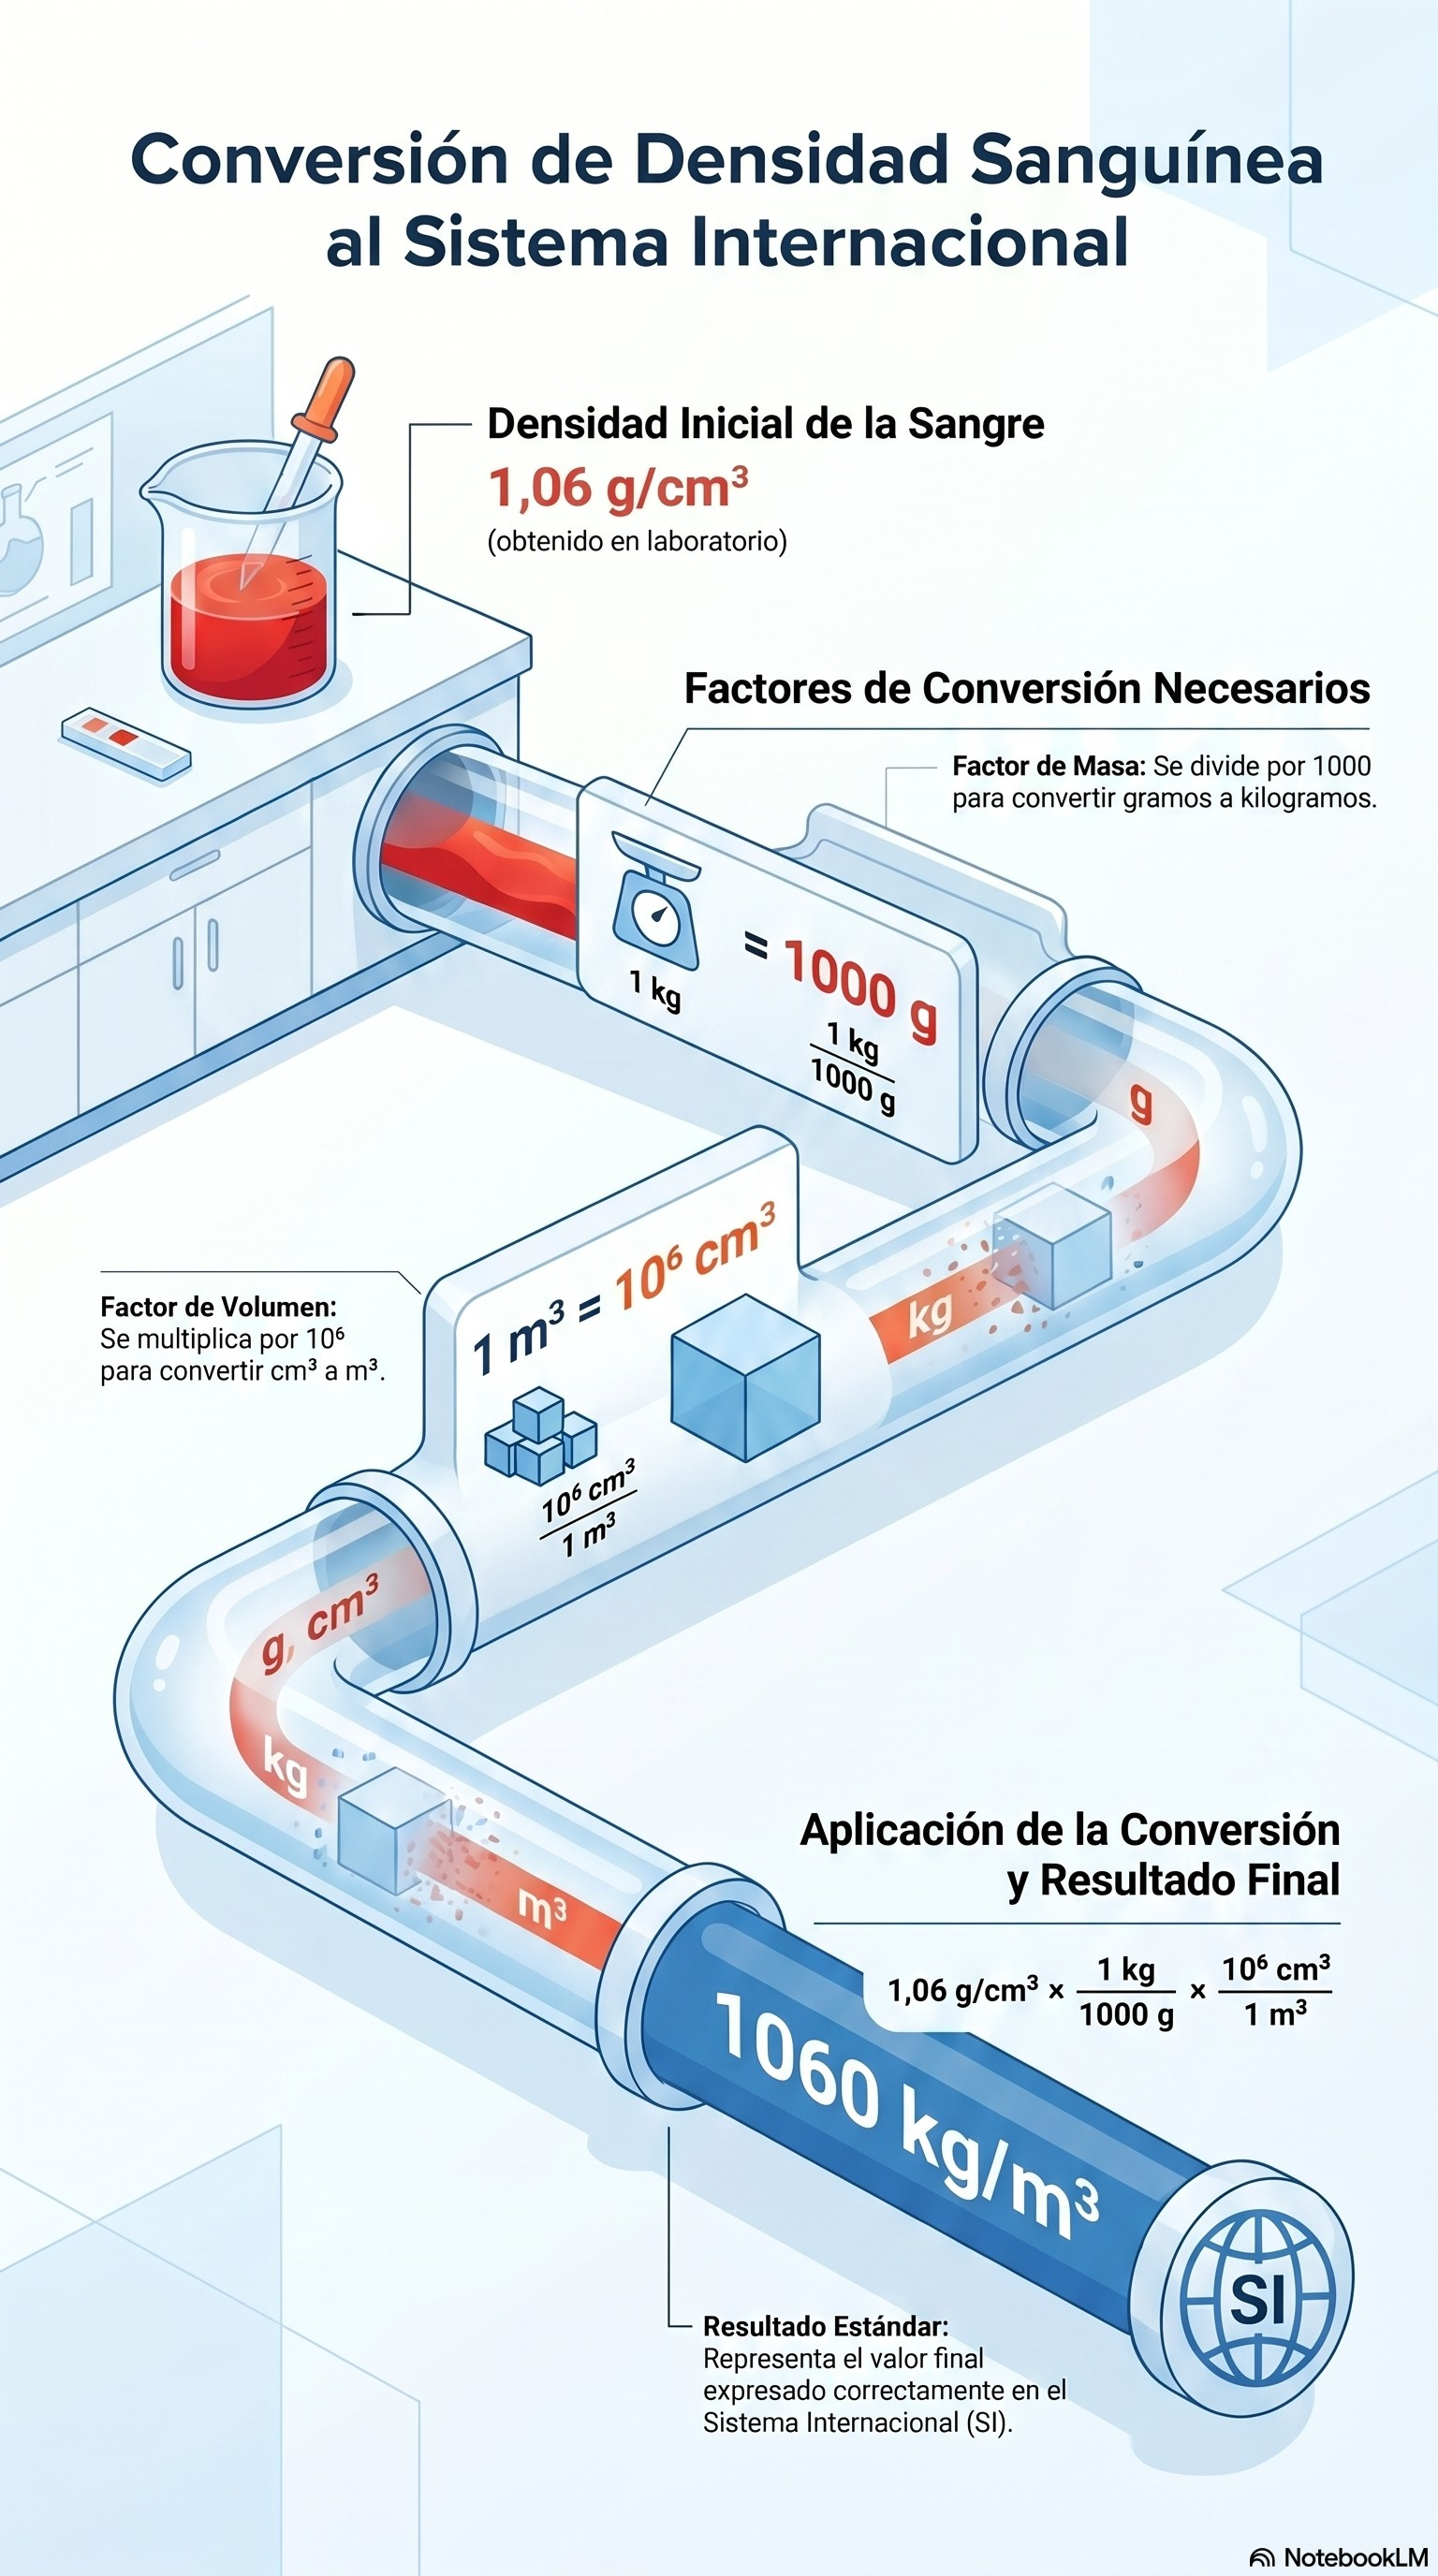
\includegraphics[width=0.6\textwidth]{prob-21.jpg}
    \end{center}
    
    \item \textbf{Sistemas de unidades (Caudal Cardíaco):} El corazón de un adulto sano bombea aproximadamente $5$ litros de sangre por minuto en reposo. Exprese este caudal en metros cúbicos por segundo ($\text{m}^3\text{/s}$) empleando notación científica.
    \textbf{Solución:} \\
    Sabiendo que $1 \text{ L} = 10^{-3} \text{ m}^3$ y $1 \text{ min} = 60 \text{ s}$:
    \[ Q = \frac{5 \text{ L}}{\text{min}} = \frac{5 \times 10^{-3} \text{ m}^3}{60 \text{ s}} \approx 8.33 \times 10^{-5} \, \frac{\text{m}^3}{\text{s}} \]
    \begin{center}
        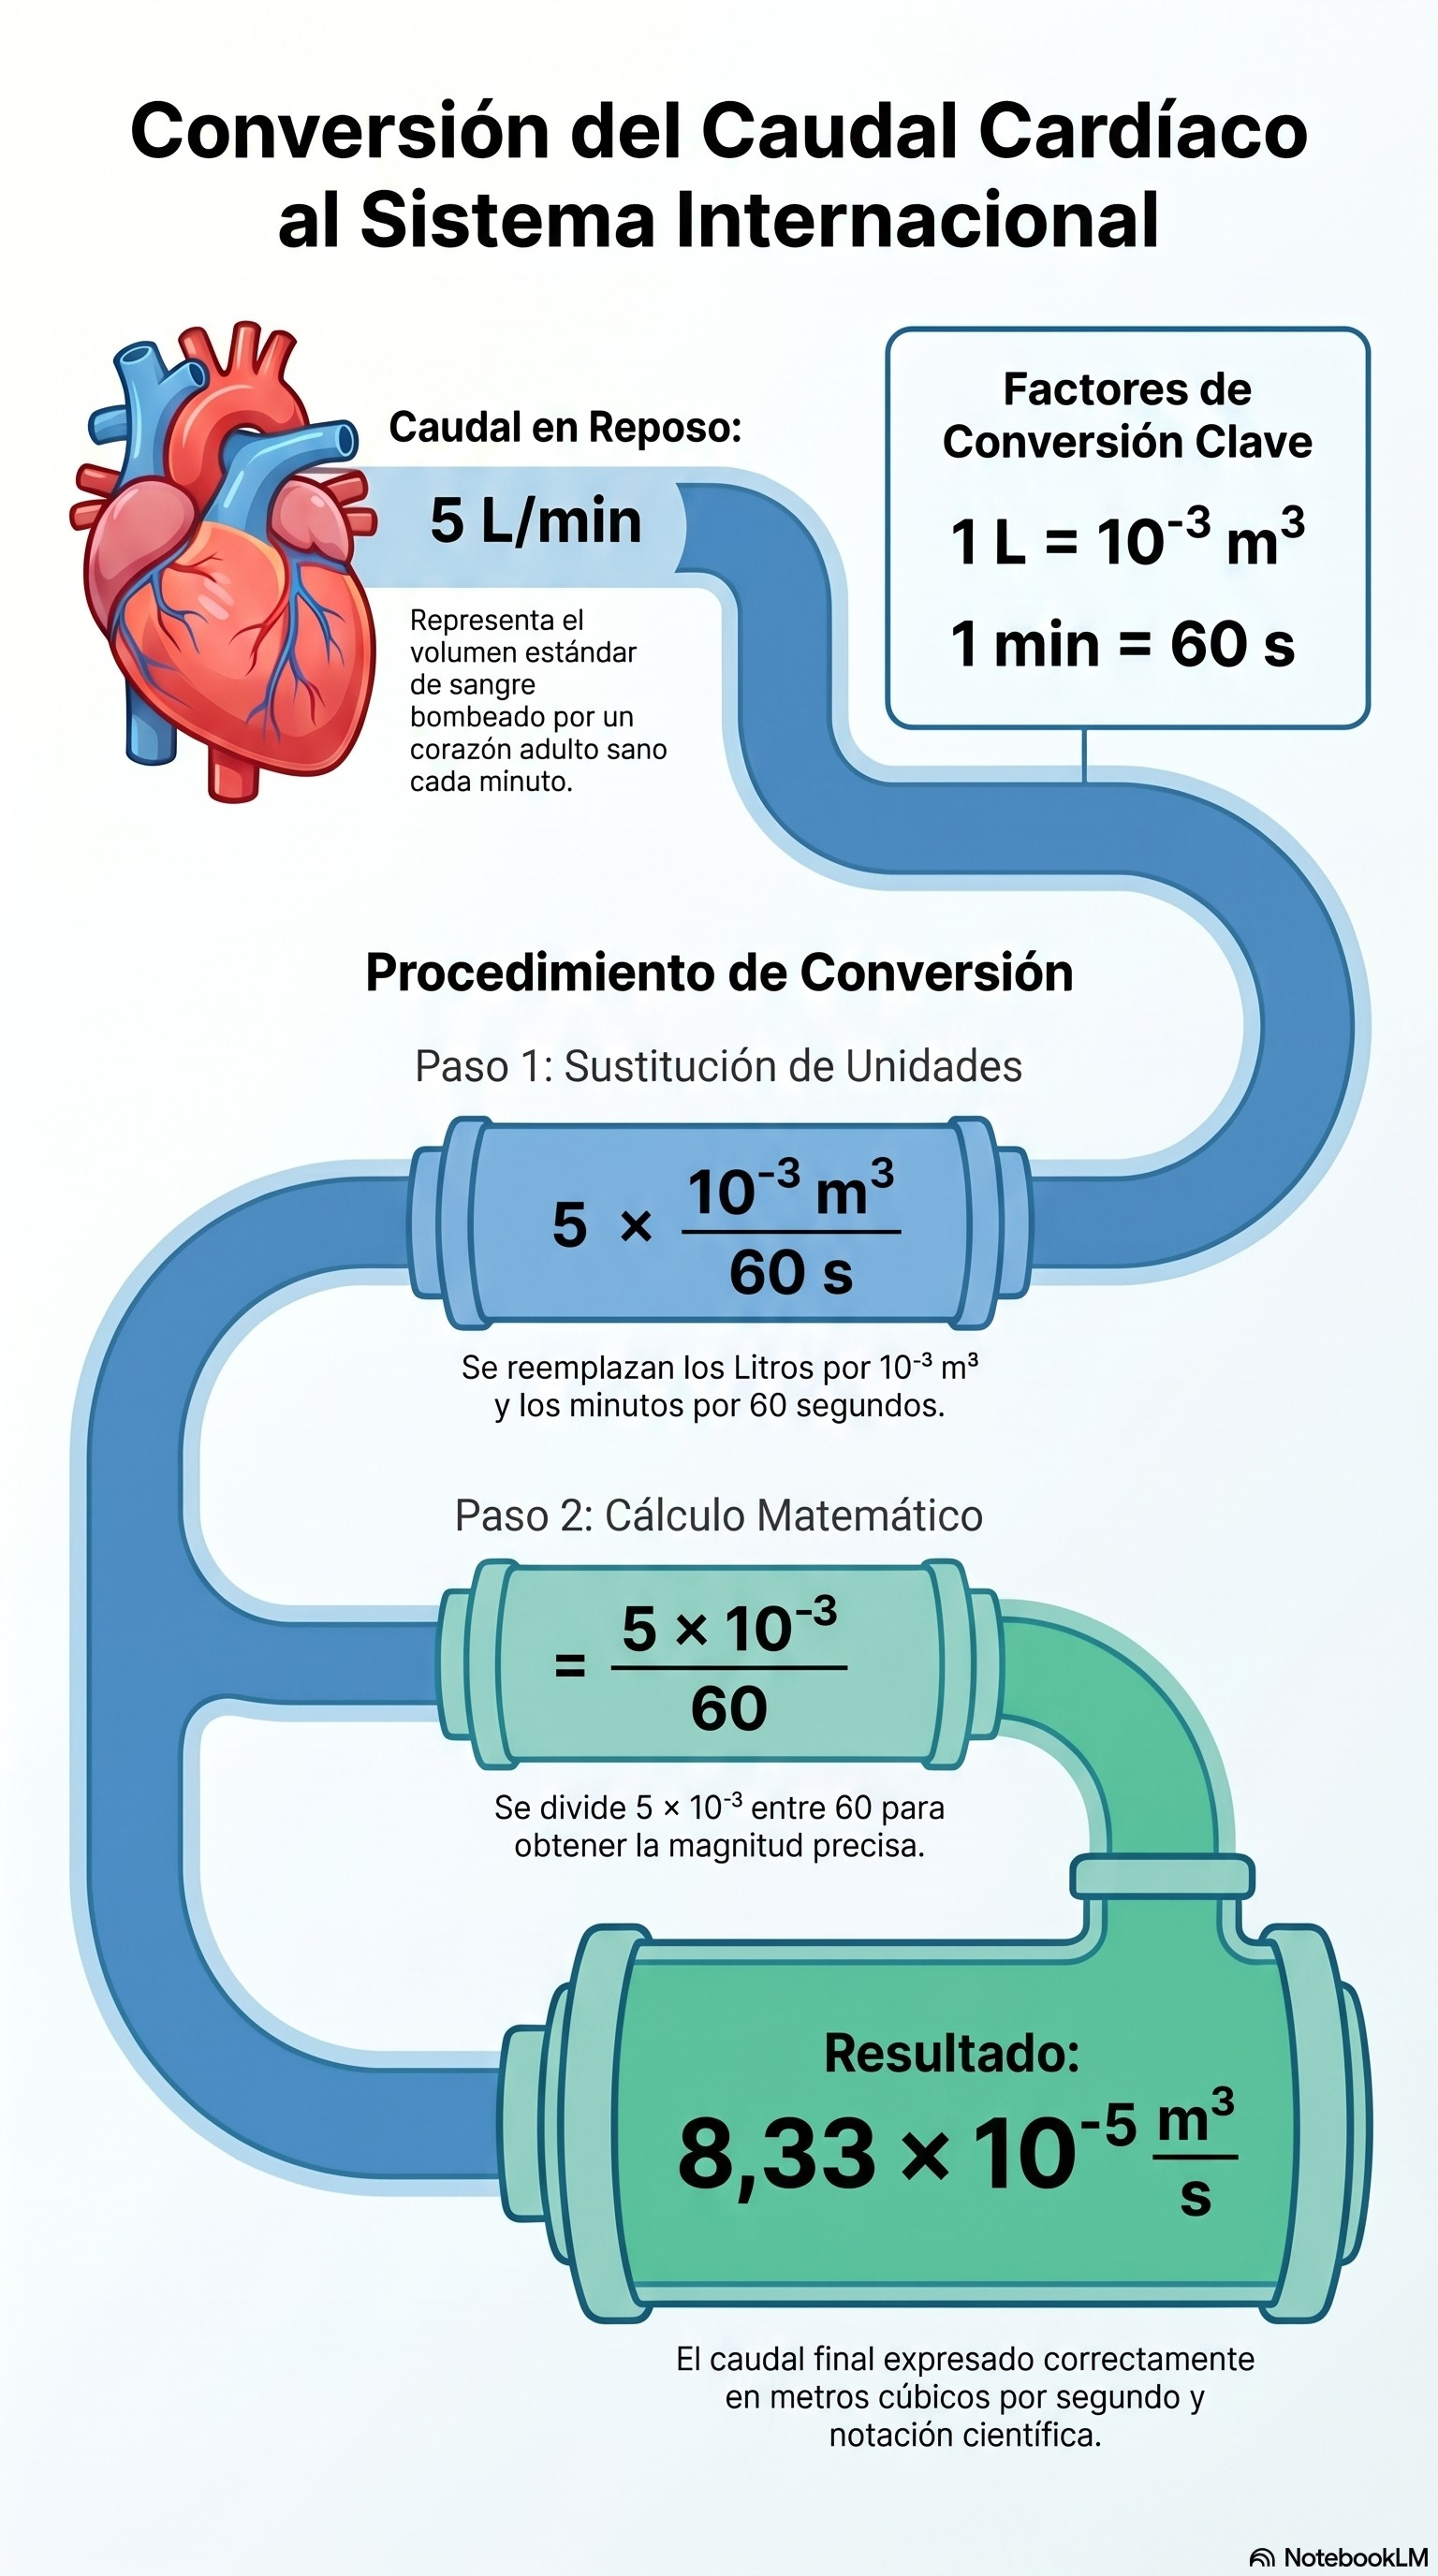
\includegraphics[width=0.6\textwidth]{prob-22.jpg}
    \end{center}

    \item \textbf{Sistemas de unidades (Presión Arterial):} La presión sistólica normal es de unos $120$ mmHg (milímetros de mercurio). Conociendo que $1 \text{ mmHg} \approx 133.322 \text{ Pa}$ (Pascales, medida del Sistema Internacional), convierta la presión sistólica a Pascales.
    \textbf{Solución:} \\
    \[ P = 120 \text{ mmHg} \times \left( \frac{133.322 \text{ Pa}}{1 \text{ mmHg}} \right) = 15998.64 \text{ Pa} \approx 1.6 \times 10^4 \text{ Pa} \]
    \begin{center}
        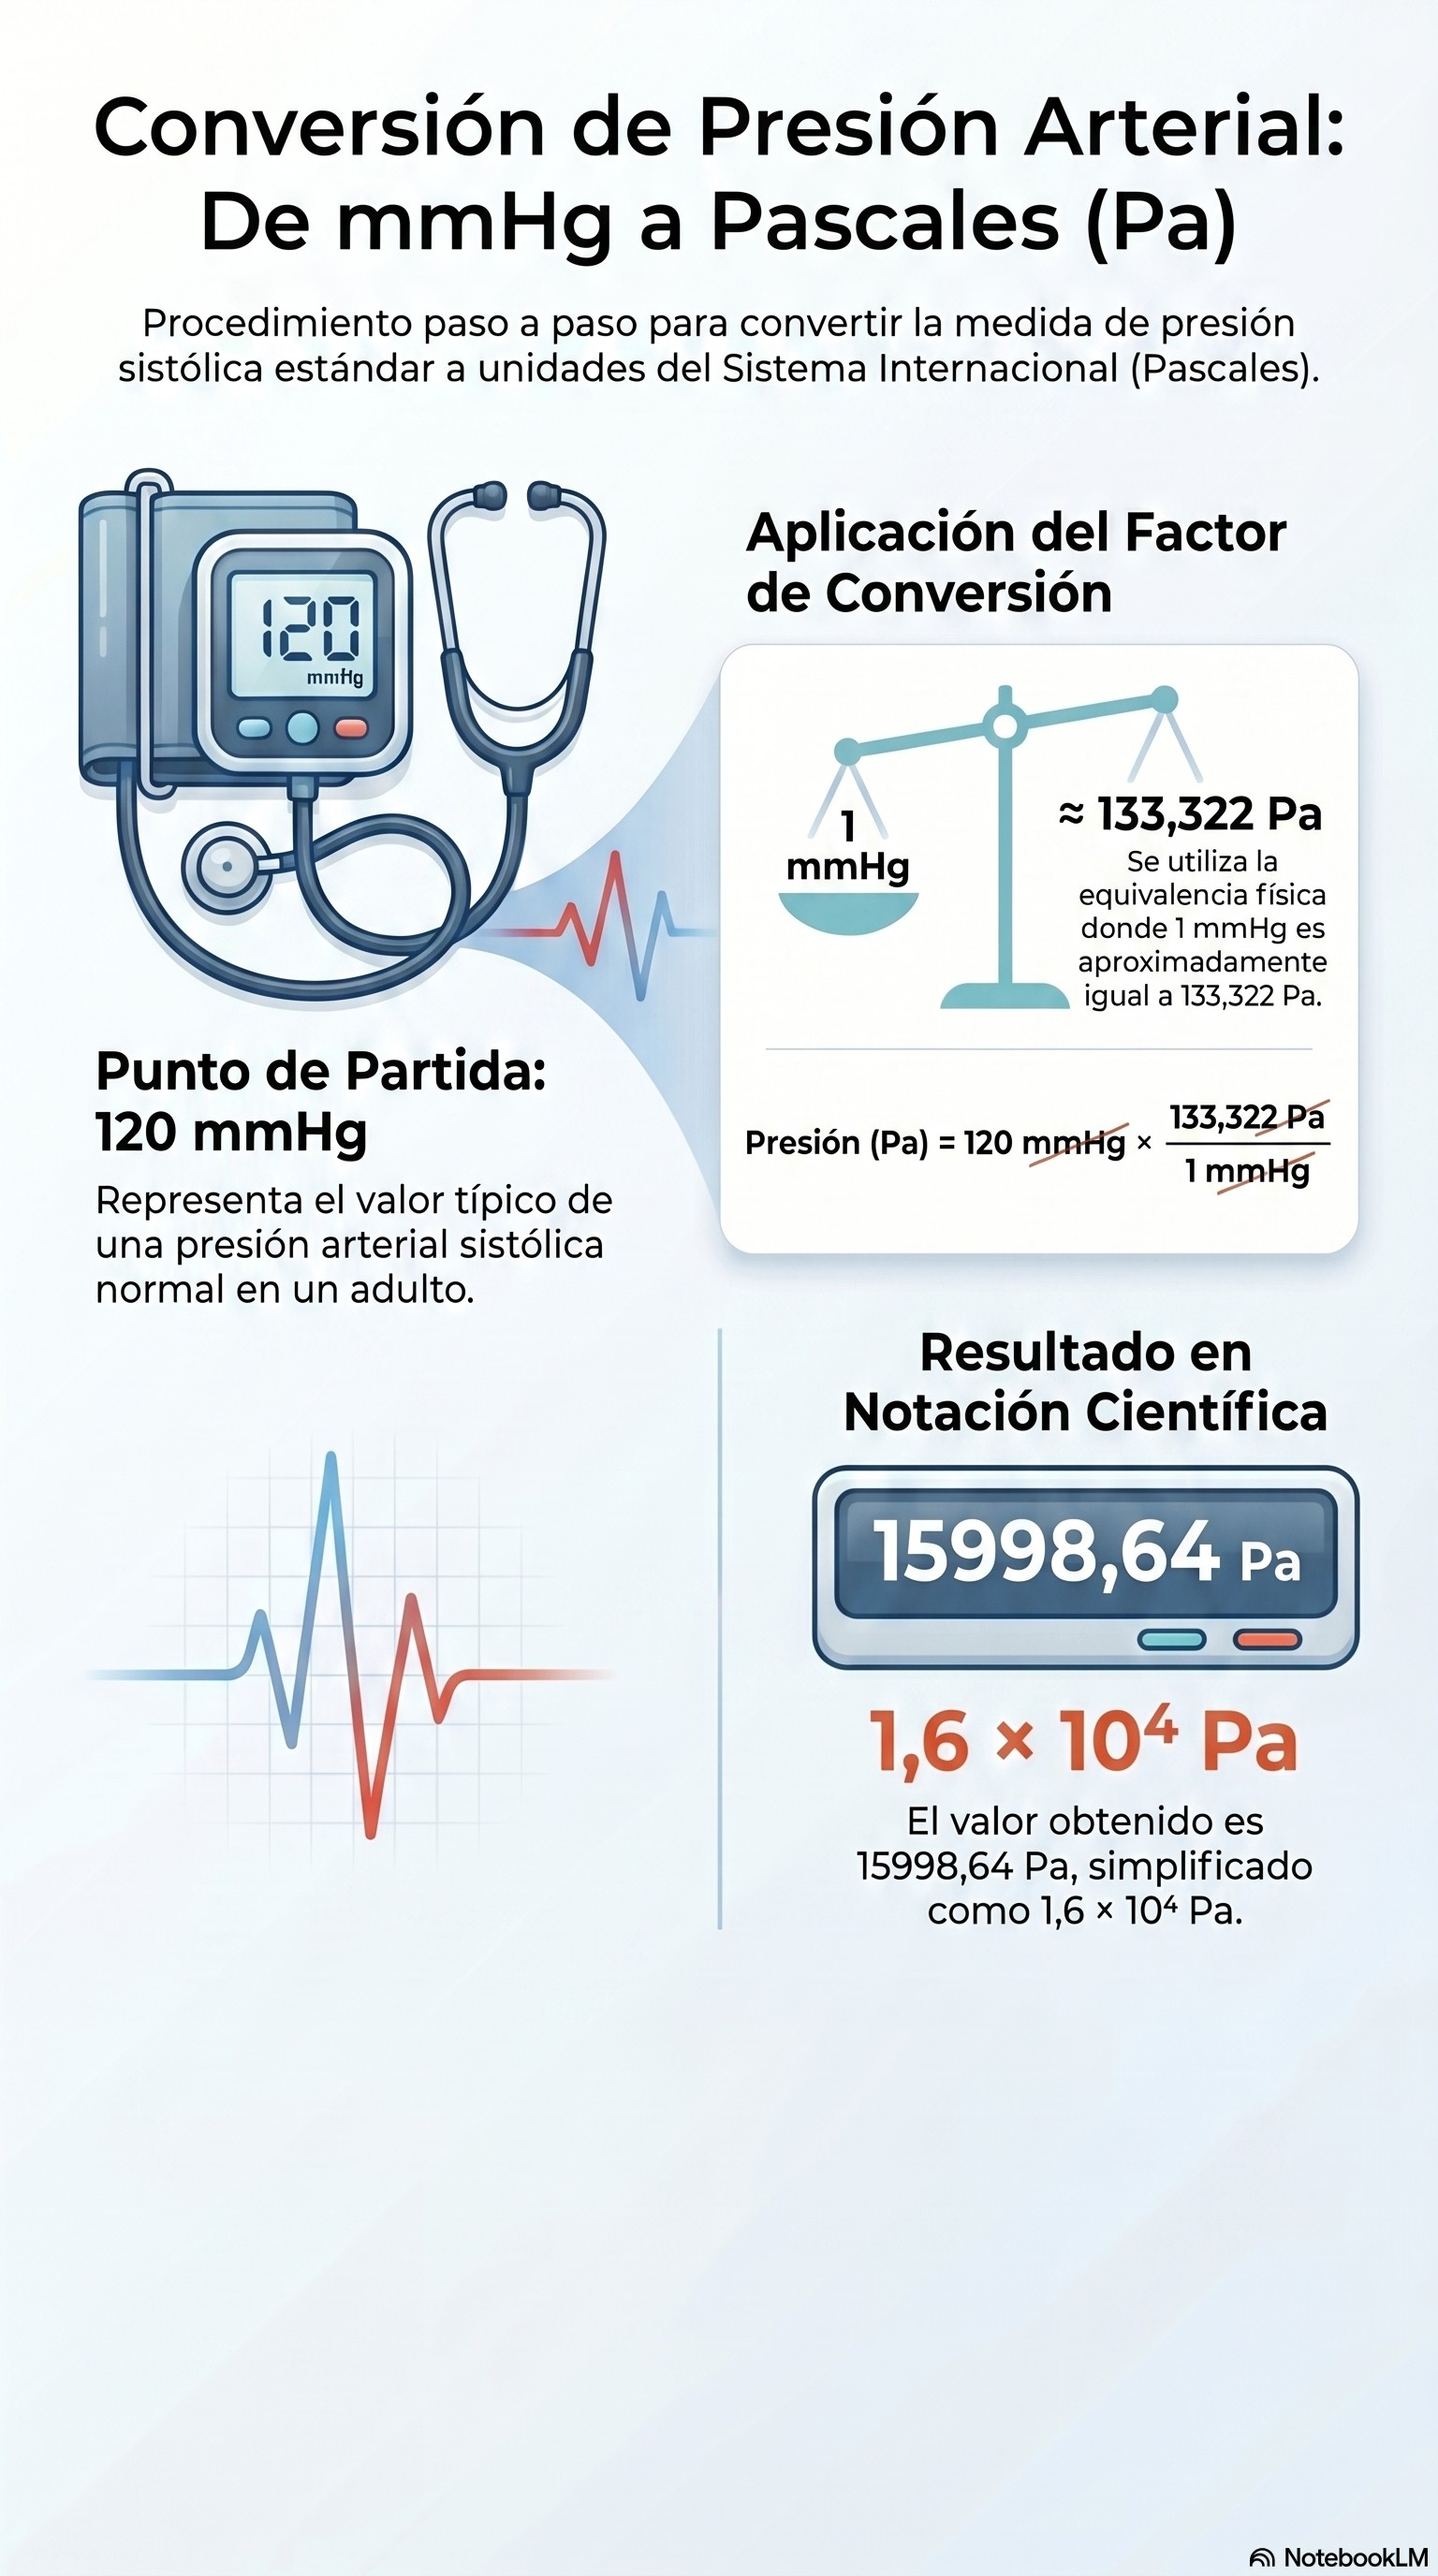
\includegraphics[width=0.6\textwidth]{prob-23.jpg}
    \end{center}

    \item \textbf{Sistemas de unidades (Velocidad de Flujo):} La velocidad media del flujo sanguíneo en la aorta humana es de aproximadamente $30$ cm/s. Convierta esta velocidad a metros por hora ($\text{m/h}$).
    \textbf{Solución:} \\
    Usamos los factores $1 \text{ m} = 100 \text{ cm}$ y $1 \text{ h} = 3600 \text{ s}$:
    \[ v = 30 \, \frac{\text{cm}}{\text{s}} \times \left( \frac{1 \text{ m}}{100 \text{ cm}} \right) \times \left( \frac{3600 \text{ s}}{1 \text{ h}} \right) = 30 \times 0.01 \times 3600 = 1080 \, \frac{\text{m}}{\text{h}} \]
    \begin{center}
        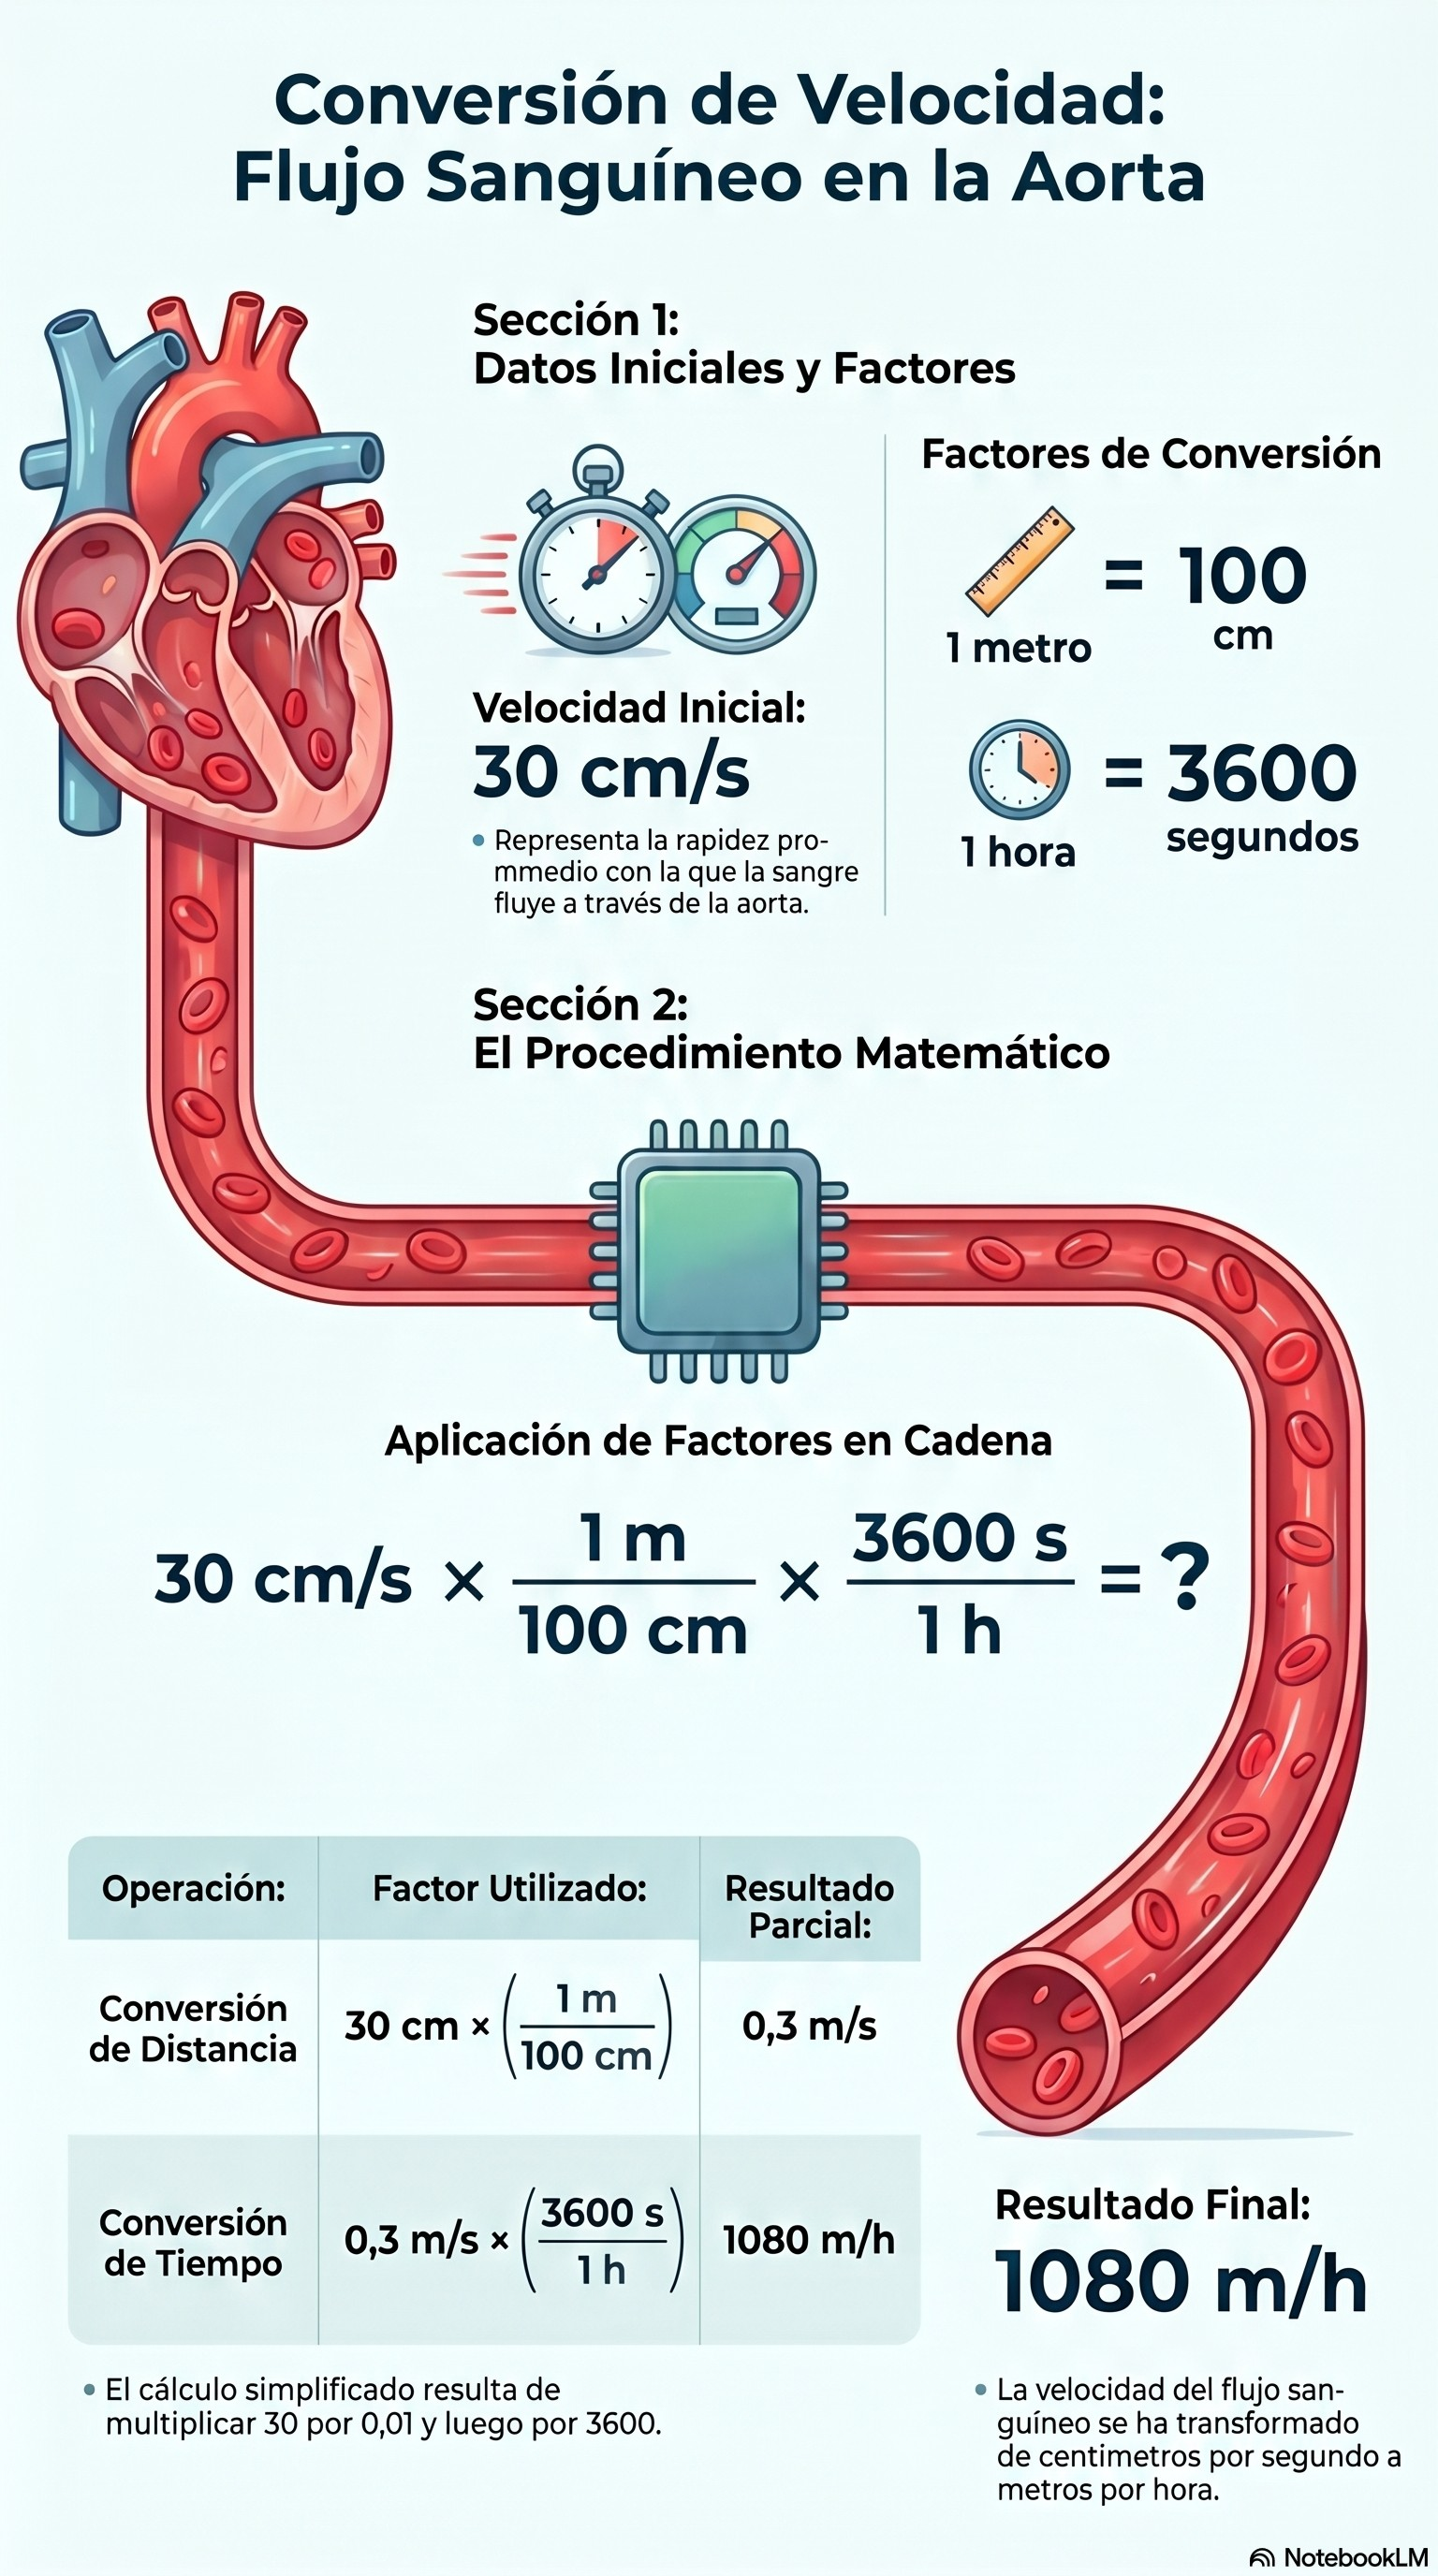
\includegraphics[width=0.6\textwidth]{prob-24.jpg}
    \end{center}

    \item \textbf{Sistemas de unidades (Dosis Médica por Peso):} Un paciente recibe un medicamento a razón de $5$ mg por cada kg de peso corporal. Si en el expediente clínico el paciente registra un peso de $154$ libras (lb). Sabiendo que $1 \text{ kg} \approx 2.2 \text{ lb}$, ¿cuántos miligramos del medicamento debe recibir?
    \textbf{Solución:} \\
    Primero calculamos el peso en kg:
    \[ \text{Peso en kg} = 154 \text{ lb} \times \left( \frac{1 \text{ kg}}{2.2 \text{ lb}} \right) = 70 \text{ kg} \]
    Luego determinamos la dosis total:
    \[ \text{Dosis total} = 70 \text{ kg} \times \left( \frac{5 \text{ mg}}{1 \text{ kg}} \right) = 350 \text{ mg} \]
    \begin{center}
        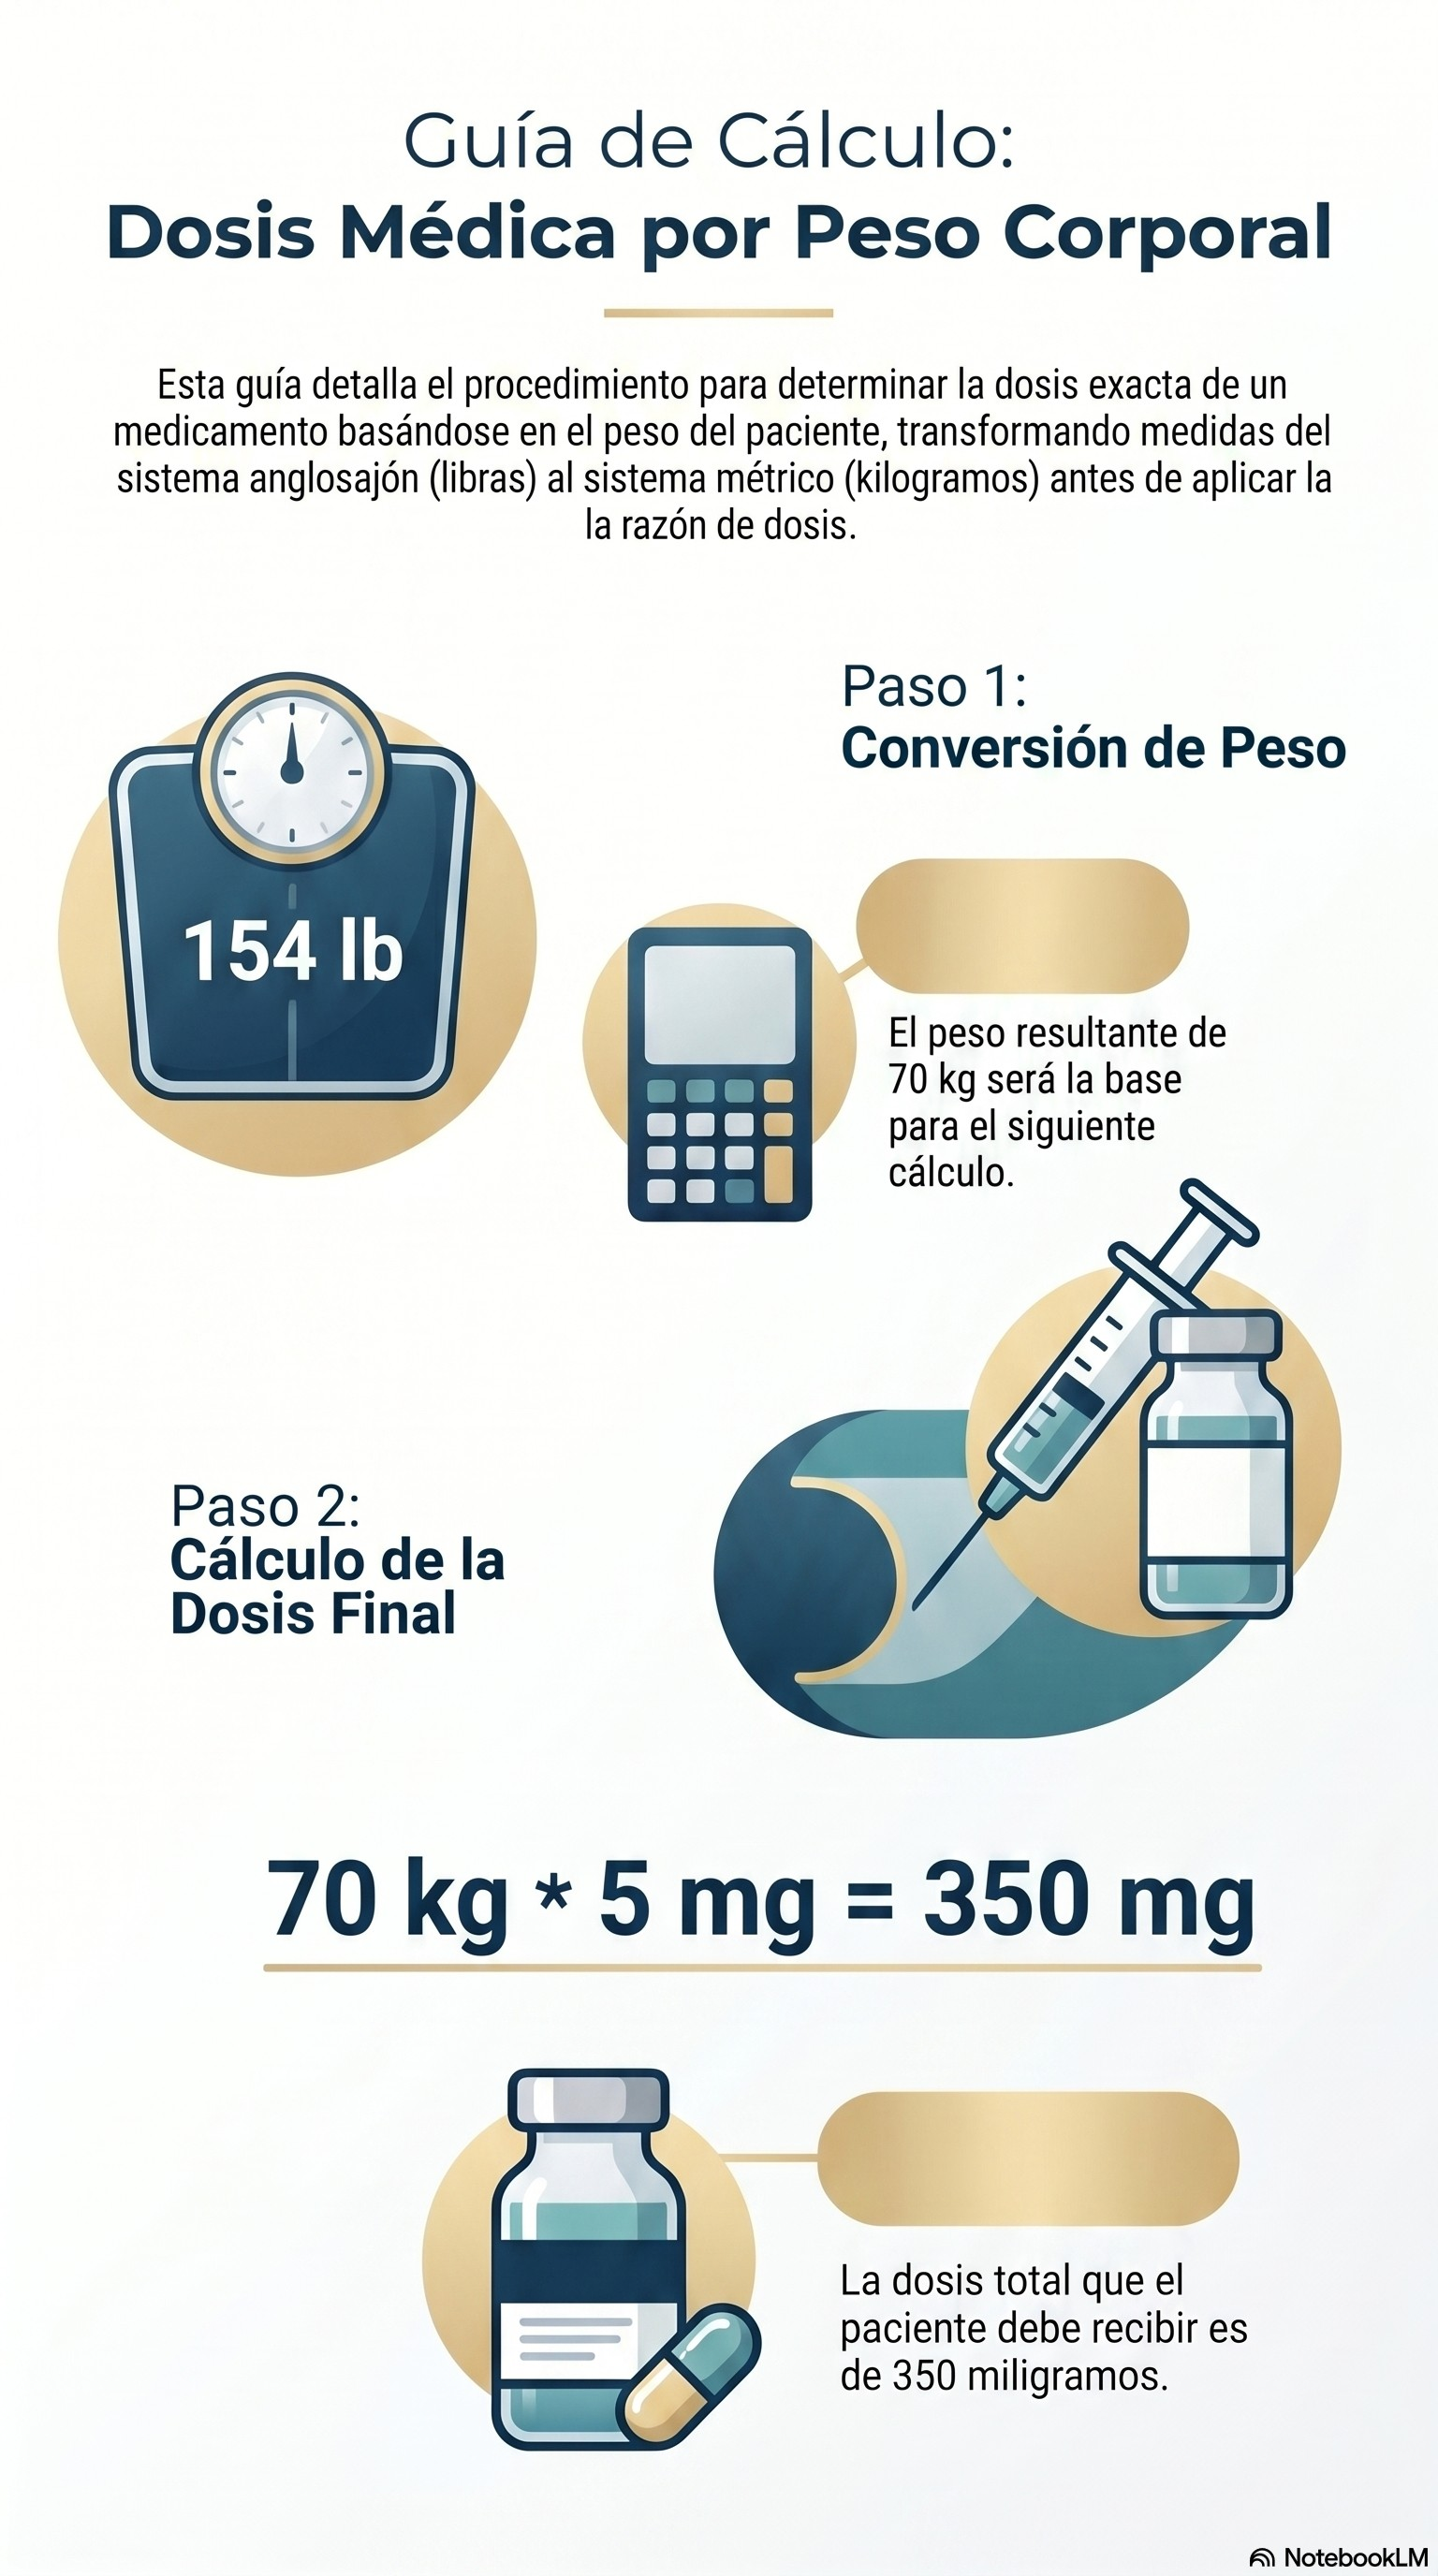
\includegraphics[width=0.6\textwidth]{prob-25.jpg}
    \end{center}

\end{enumerate}

\end{document}